% =====================================================================
% AUTHORITATIVE MANUSCRIPT — ATLAS Open Data Record 80030
% Revision 2, built 2026-09-09 from the frozen analysis artifacts only,
% incorporating the seventeen points of the external revision checklist.
% Revision 3, 2026-10-10: adds the robustness extension (paired Poisson
% bootstrap, six-seed study, per-jet input response, scale-free input sets)
% read from 04_Results/{stat_bootstrap,tagger_variants,feature_response}_round1,
% and the dataset-README statements in sources/. No frozen number is changed.
% Reconstruction fingerprint : c28a262540824e9db90f34c421f10c70
% Final model SHA-256        : 63a23308efbf2ce90418c8e657730f571db4798fc9ca2fb3692cb986de405f4c
% Metrics source             : final_metrics_atlas_tagger_xgb_final_production_round1_round1.json
% SHAP source                : shap_delta_final_production_round3
% Conformal source           : conformal_coverage_round1
% Companion file             : atlas80030_supplementary.tex
%
% Template: Springer Nature sn-jnl with the [iicol] option, which is what the
% EPJ C submission guidelines ask for ("We recommend using Springer Nature's
% LaTeX template and choosing the formatting option '[iicol]'").  The abstract
% is inside the 150-250 word range that the same guidelines set.
% =====================================================================
\PassOptionsToPackage{table}{xcolor}
\documentclass[pdflatex,sn-mathphys,Numbered,iicol]{sn-jnl}

\usepackage{graphicx}
\usepackage{booktabs}
\usepackage{array}
\usepackage{amsmath,amssymb}
\usepackage{url}
\usepackage{iftex}
\ifPDFTeX
  \usepackage[protrusion=true,expansion=true]{microtype}
\else
  \usepackage[protrusion=true,expansion=false]{microtype}
\fi
\providecommand{\citep}{\cite}\providecommand{\citet}{\cite}

% Title-page e-mail block: print the contributing authors first and the
% corresponding author last, reversing the class default.  The class file
% itself is left unmodified.
\usepackage{etoolbox}
\makeatletter
\patchcmd{\@maketitle}%
  {\ifx\corrauthemail\@empty\else{\ifnum\aucount>1*\fi}Corresponding author(s). E-mail(s): \corrauthemail\par\fi\ifx\authemail\@empty\else Contributing authors:\ \authemail\fi}%
  {\ifx\authemail\@empty\else Contributing authors:\ \authemail\par\fi\ifx\corrauthemail\@empty\else{\ifnum\aucount>1*\fi}Corresponding author(s). E-mail(s): \corrauthemail\fi}%
  {}{\PackageWarning{atlas80030}{Could not reorder the title-page e-mail block}}
\makeatother

% Stop LaTeX stretching the vertical glue between paragraphs to force equal
% column depth; uneven column bottoms are preferable to uneven paragraph gaps.
\raggedbottom
\setlength{\emergencystretch}{2em}

\newcommand{\pt}{p_{\mathrm{T}}}
\newcommand{\dR}{\Delta R}

\begin{document}

\title[Systematic robustness of a boosted top tagger on ATLAS open data]{Systematic
robustness of a boosted top-quark tagger on ATLAS open data: a constituent-level
feature reconstruction, paired SHAP-Delta attribution drift, and conformal coverage}

\author[1]{\fnm{Adeel} \sur{Rahmat}}\email{adeelrahmat64@gmail.com}
\author[1]{\fnm{M. Imran} \sur{Jamil}}\email{imran.jamil@umt.edu.pk}
\author*[1]{\fnm{Ahmed} \sur{Awan}}\email{h.ahmadawan@gmail.com}
\affil[1]{\orgdiv{Department of Physics}, \orgname{University of Management and
Technology}, \orgaddress{\street{C-II Johar Town}, \city{Lahore}, \postcode{54770},
\country{Pakistan}}}

\abstract{The ATLAS top-tagging open dataset releases detector-systematic and
generator-modelling variations as dedicated simulated samples rather than as
per-event weights. For the four exactly pairable calorimeter variations, the
fifteen stored high-level substructure quantities remain nominal, so we
recompute them from the released constituents with a single implementation. Against the stored
nominal branches the median relative agreement is $2.5\times10^{-8}$ to
$4.8\times10^{-7}$ per quantity on 14{,}103 jets; the $0.072\%$ of comparisons
beyond a $10^{-3}$ tolerance fall on 44 jets, none of them a formula or
implementation mismatch. The frozen reconstruction was applied
to 80{,}481{,}421 jet entries. An XGBoost tagger developed from a five-million-jet nominal subset
reaches an unweighted area under the receiver-operating-characteristic curve of
$0.9320$ and background rejection $41.91 \pm 0.12$ (stat.) at $50\%$ signal
efficiency on 10{,}306{,}812 test jets. Its total relative systematic uncertainty
is $(25.8 \pm 0.6_{\mathrm{stat}} \pm 0.5_{\mathrm{seed}})\%$, dominated by
generator modelling ($20.0\%$). Under the calorimeter energy-scale and
energy-resolution variations, paired TreeSHAP attribution drift is led by ECF$_3$,
the input of highest degree in the constituent momenta, while global importance
orderings change minimally (Spearman $\rho \ge 0.986$). Restricting the tagger to
dimensionless inputs lowers the six-seed mean total uncertainty from $26.3\%$ to
$15.8\%$ but background rejection from $41.8$ to $18.9$. Class-conditional split-conformal
coverage, calibrated once on nominal simulation, stays within one percentage point
of the $90\%$ target on all nine detector-systematic samples.}

\keywords{jet substructure, boosted top tagging, machine learning, SHAP, conformal
prediction, systematic uncertainties, ATLAS open data}

\maketitle

% =====================================================================
\section{Introduction}
\label{sec:intro}

Identifying boosted top quarks from their hadronic decays is among the harder
jet-tagging problems at the Large Hadron Collider~\cite{Evans2008}. When a top quark is
produced with transverse momentum well above its rest mass of about
$173$~GeV~\cite{PDG2024}, the three quarks from $t \to Wb \to qqb$ merge into a single
large-radius jet whose interior carries a three-pronged radiation pattern. Separating
such jets from the far more abundant QCD multijet background matters both for
measurements of boosted top-pair production and for searches involving top quarks.

Early taggers cut on individual substructure observables such as $N$-subjettiness
ratios~\cite{Thaler2011,Thaler2012} or energy correlation
functions~\cite{Larkoski2013}. Multivariate combinations followed, and deep networks
reading low-level constituent information pushed background rejection substantially
higher~\cite{Kasieczka2019,Qu2020,Komiske2019}; Refs.~\cite{Larkoski2020,Guest2018}
review that progression. ATLAS and CMS have both published systematic studies of
boosted-top classifiers on full detector simulation~\cite{ATLAS2024,CMS2020}. The most
recent ATLAS study~\cite{ATLAS2024} benchmarked several architectures and released the
underlying simulation as an open dataset~\cite{ATLASOpenData2024}, together with a
prescribed procedure for turning tagger performance into a systematic uncertainty.

That release is unusual in one respect that shapes this paper. Detector systematic
variations and generator-modelling alternatives are distributed as \emph{separate
simulated samples}, not as per-event weights. A weight-based analysis of tagger
robustness is therefore not available on this dataset. In the four calorimeter
variations that pair exactly, all fifteen stored high-level quantities remain
nominal despite changed constituents (Section~\ref{sec:stale}). A study of how
a classifier responds to these variations must first rebuild the feature space
from the released constituents.

The contributions of this work are the following.
\begin{enumerate}
\item \emph{A reconstructed feature space.} All fifteen high-level quantities are
  rebuilt from the released constituents with one implementation applied identically
  on both sides of every comparison, validated against the stored nominal branches,
  and applied to 80.5 million jet entries (Section~\ref{sec:data}). This is the
  enabling step for everything that follows.
\item \emph{A benchmarked tagger with measured precision.} An XGBoost
  tagger~\cite{Chen2016,Friedman2001} is trained on that feature space and evaluated
  exactly as ATLAS prescribes for this dataset, so that its performance and systematic
  uncertainty are directly comparable to the published benchmark. The statistical
  uncertainty of the nominal performance and of every systematic uncertainty is
  measured with a bootstrap that preserves the jet-by-jet pairing of the calorimeter variations, and its
  dependence on the training seed with six independent fits
  (Section~\ref{sec:precision}).
\item \emph{Paired attribution drift.} A \emph{paired} analysis of Shapley additive
  explanations (SHAP)~\cite{Lundberg2017,Lundberg2020trees} measures how the
  attribution assigned to each feature moves for the \emph{same physical jet} under a
  systematic variation.
\item \emph{An explanation in terms of the inputs.} The leading attribution drift
  and the dominant detector and modelling uncertainties are traced to the degree of
  each input in the constituent momenta, by measuring the per-jet response of every input and by retraining on
  dimensionless inputs (Section~\ref{sec:degreemethod}).
\item \emph{Coverage under systematic variation.} A class-conditional split-conformal
  coverage check~\cite{Vovk2005,Angelopoulos2023} asks whether prediction sets
  calibrated once on nominal simulation retain their nominal coverage on varied
  simulation.
\end{enumerate}

The two diagnostics operate at different levels, and it is worth being explicit about
that from the start. The SHAP analysis is genuinely paired: it is restricted to the
four calorimeter-cluster variations whose jets match the nominal sample one for one on
an exact identity key, so each attribution difference is a difference for one physical
jet. The conformal analysis is not paired. It is a dataset-level comparison in which
one fixed pair of thresholds, calibrated once on held-out nominal simulation, is
applied unchanged to the nominal test sample and to all nine detector-systematic
samples, including the four track samples that are different jet populations
altogether. Neither technique is new in itself: tagger robustness under detector
systematics~\cite{ATLAS2024,CMS2020,Sahu2024}, Shapley attributions for boosted-top
classifiers~\cite{Bhattacherjee2024,Sahu2024}, and conformal prediction in high-energy
physics~\cite{Araz2025} have all been reported before. What is new here is that the
attribution comparison is made on physically matched jet pairs drawn from dedicated
systematic samples, on a feature space rebuilt so that the two sides of each comparison
are genuinely comparable; that the uncertainty budget of the prescribed procedure is
given with its own statistical precision; that the leading attribution drift and the
dominant uncertainties are explained, and tested by an intervention on the inputs,
through a property of the input definitions; and that the coverage comparison is carried across every detector
variation the release provides.

Throughout, the published ATLAS high-level network (hlDNN) is used only as an external
reference point in the same fifteen-variable feature space. We do not attempt to
reproduce it, and we do not interpret the difference between our tagger and it as a
measurement of anything.

% =====================================================================
\section{Dataset and feature-space reconstruction}
\label{sec:data}

\subsection{ATLAS Open Data Record 80030}
\label{sec:record}

The ATLAS top-tagging open dataset~\cite{ATLASOpenData2024} is built from simulated
proton--proton collisions at $\sqrt{s}=13$~TeV passed through the full ATLAS detector
simulation~\cite{ATLASDetector2008} in GEANT4~\cite{Agostinelli2003}. Signal jets come
from a hypothetical $Z' \to t\bar t$ resonance with $m_{Z'} = 2$~TeV generated with
PYTHIA~8~\cite{Sjostrand2015}, reweighted at generation to populate the jet $\pt$ range
$0.35$--$5$~TeV approximately uniformly; background jets come from QCD light-quark and
gluon production~\cite{ATLAS2024}. Jets are clustered with the anti-$k_{\mathrm{T}}$
algorithm~\cite{Cacciari2008anti} at $R = 1.0$ using FastJet~\cite{Cacciari2012fastjet}.
Each entry stores the four-vectors of up to 200 jet constituents, the jet four-vector,
fifteen high-level substructure quantities, a signal/background label, and, for the
nominal samples only, a training weight and a vector of PYTHIA shower weights.

The release distributes three families of samples. The \emph{nominal} family supplies
training and testing jets. Nine \emph{detector-systematic} families apply a single
detector variation to the constituents: cluster energy scale up and down
(\texttt{esup}, \texttt{esdown}), cluster energy resolution (\texttt{cer}), cluster
position resolution (\texttt{cpos}), track efficiency in two configurations
(\texttt{teg}, \texttt{tej}), track fake rate in two configurations (\texttt{tfl},
\texttt{tfj}), and track momentum bias (\texttt{bias})~\cite{ATLAS2024}. Six
\emph{modelling} families replace generator components: matrix-element and
parton-shower matching for the signal (\texttt{ttbar\_pythia} against
\texttt{ttbar\_herwig}), the Herwig~7 angular-ordered against dipole parton shower for
the background (\texttt{angular} against \texttt{dipole})~\cite{Bellm2016}, and the
Sherpa~2.2 cluster against Lund-string hadronisation model for the background
(\texttt{cluster} against \texttt{string})~\cite{Bothmann2019}.

Table~\ref{tab:datasets} lists the seventeen samples processed here, with the file and
row counts recorded by the read-only cache integrity audit. In total
\textbf{80{,}481{,}421 jet entries} were read and reconstructed. The released
\texttt{train\_nominal} partition is far larger than the subset used here; we use
$5{,}000{,}000$ of its jets, a choice discussed in
Sections~\ref{sec:training} and~\ref{sec:limitations}. Each detector-systematic sample
enters the evaluation with $5{,}000{,}000$ jets, of which at most 244 fail the
eligibility rule of Section~\ref{sec:training}; this is the size the dataset
documentation recommends as a minimum in evaluation when the experimental
uncertainties are calculated~\cite{ATLASGitLab}.

\begin{table}[t]
\centering\small
\caption{The seventeen samples processed in this work, with the number of released
  HDF5 files and jet entries in each. Counts are taken from the read-only cache
  integrity audit, which verified file-by-file and row-by-row agreement between every
  source file and its reconstructed feature cache. The total is
  $80{,}481{,}421$ jet entries in 810 cache files.}
\label{tab:datasets}
\begin{tabular}{llrr}
\toprule
Family & Sample & Files & Jet entries \\
\midrule
Nominal   & \texttt{train\_nominal} & 50  & 5{,}000{,}000 \\
          & \texttt{test\_nominal}  & 104 & 10{,}306{,}813 \\
\midrule
Detector  & \texttt{esup}    & 50 & 5{,}000{,}000 \\
          & \texttt{esdown}  & 50 & 5{,}000{,}000 \\
          & \texttt{cer}     & 50 & 5{,}000{,}000 \\
          & \texttt{cpos}    & 50 & 5{,}000{,}000 \\
          & \texttt{teg}     & 50 & 5{,}000{,}000 \\
          & \texttt{tej}     & 50 & 5{,}000{,}000 \\
          & \texttt{tfl}     & 50 & 5{,}000{,}000 \\
          & \texttt{tfj}     & 50 & 5{,}000{,}000 \\
          & \texttt{bias}    & 50 & 5{,}000{,}000 \\
\midrule
Modelling & \texttt{ttbar\_pythia} &  2 &   193{,}792 \\
          & \texttt{ttbar\_herwig} &  2 &   180{,}811 \\
          & \texttt{cluster}       & 51 & 5{,}000{,}004 \\
          & \texttt{string}        & 51 & 5{,}000{,}001 \\
          & \texttt{angular}       & 50 & 4{,}900{,}000 \\
          & \texttt{dipole}        & 50 & 4{,}900{,}000 \\
\midrule
\multicolumn{2}{l}{\textbf{Total}} & \textbf{810} & \textbf{80{,}481{,}421} \\
\bottomrule
\end{tabular}
\end{table}

\subsection{The fifteen high-level quantities}
\label{sec:hlq}

We use the fifteen high-level quantities of Table~3 of Ref.~\cite{ATLAS2024}:
$N$-subjettiness $\tau_1$--$\tau_4$ computed on winner-take-all $k_{\mathrm{T}}$
axes~\cite{Thaler2011,Thaler2012,Larkoski2014WTA}; the $k_{\mathrm{T}}$ splitting
scales $\sqrt{d_{12}}$ and $\sqrt{d_{23}}$~\cite{Thaler2008}; the energy correlation functions
ECF$_1$, ECF$_2$, ECF$_3$ and the ratios $C_2$~\cite{Larkoski2013} and
$D_2$~\cite{Larkoski2014PC,Larkoski2016D2}; the generalised energy-correlation ratios $L_2$ and $L_3$
built from the observables of Ref.~\cite{Moult2016} in the combination specified by
ATLAS~\cite{ATLASPub2021}; the minimum pairwise subjet mass
$Q_w$~\cite{Kaplan2008}; and the jet thrust major~\cite{Chen2012}. No kinematic variable such as jet
$\pt$ or mass enters the classifier, which keeps the feature space identical to the
published high-level baseline.

\subsection{Why the released high-level branches cannot be used}
\label{sec:stale}

The fifteen high-level branches are present in the systematically varied files, and a
weight- or branch-based robustness study would naturally read them. In the four
calorimeter-cluster samples for which exact jet pairing is valid, they do not carry
the variation. Against \texttt{test\_nominal}, \texttt{esup}, \texttt{esdown} and
\texttt{cpos} each have $5{,}000{,}000$ exact matches, and \texttt{cer} has
$4{,}995{,}059$. For every valid matched jet, all fifteen stored high-level values
are float32 bit-identical to their nominal counterparts. The released constituents
nevertheless differ: the relative summed-constituent-$\pt$ shift under
\texttt{esup} has mean $+6.780753\%$ and median $+7.406764\%$; under
\texttt{esdown} its mean is $-6.780749\%$ and median $-7.406822\%$.
The \texttt{cer} summed-energy response has an RMS of $3.770123\%$, while the
\texttt{cpos} constituent-centroid displacement has median
$\Delta R=4.9387\times10^{-5}$. Thus the stored high-level branches of these
four samples would conceal a real constituent-level detector variation.

The dataset documentation anticipates part of this. It states that in the samples
meant for assessing experimental systematic uncertainties the jet four-vector ``is not
re-calculated from the systematic varied jet constituents'', because the jet
four-vector is calibrated~\cite{ATLASGitLab}. It makes no corresponding statement about
the fifteen high-level quantities, which it describes only as summaries of the
constituent information. The audit shows that, in the four pairable calorimeter
samples, they behave like the jet four-vector: they are identical to their nominal
values and do not follow the varied constituents. We document this as a property of
the release rather than as an error in it, but it means that the stored branches
cannot be used to measure a tagger's response to these variations.

Because this observation is what makes the rest of the paper necessary, it is
documented sample by sample in Supplementary Table~S1. Exact-key hits in the
four track samples and \texttt{bias} are diagnostic only: their full samples do
not pass the validated one-to-one pairing criterion, so no pairwise high-level
identity fraction or same-jet constituent shift is reported for them. Their
constituent multiplicities are described as unpaired sample distributions;
\texttt{bias} has $4{,}167{,}067$ diagnostic exact-key hits but falls below the
pairing floor (Section~\ref{sec:shapmethod}).

A second point of interpretation is worth stating explicitly, because it is easy to get
wrong. The nominal files carry an \texttt{EventInfo\_mcEventWeights} array. These are
renormalisation- and factorisation-scale and PDF weights --- \emph{theory} weights.
They are not detector systematics, and the detector systematics of this release are the
dedicated samples listed in Table~\ref{tab:datasets}. In this work the shower-weight
array is used only for the four initial- and final-state-radiation scale variations of
Section~\ref{sec:syst}, exactly as the reference implementation prescribes.

\subsection{Reconstruction and closure}
\label{sec:closure}

All fifteen quantities are recomputed from the released constituent four-vectors by a
single NumPy/Numba implementation~\cite{Harris2020,Lam2015} applied identically to
every sample. Two implementation details determine whether the reconstruction closes.
Every angular separation is measured in rapidity, not pseudorapidity, matching the
convention of the FastJet interfaces~\cite{Cacciari2012fastjet} the ATLAS tools call;
because the released constituents carry non-zero mass, the two differ. And thrust
major is the ordinary three-dimensional thrust of the constituents boosted to the jet
rest frame, evaluated with the same seed-and-search policy as the ATLAS reference
implementation~\cite{ATLASGitLab}, not a transverse axis perpendicular to the thrust
axis.

The reconstruction is validated against the stored nominal branches on 14{,}103 jets
drawn from \texttt{test\_nominal} and the six modelling samples, the seven samples in
which the stored branches are meaningful. Per quantity, the median relative deviation
lies between $2.5\times10^{-8}$ (ECF$_1$) and $4.8\times10^{-7}$ ($Q_w$). Of the
$14{,}103 \times 15 = 211{,}545$ quantity--jet comparisons, 153 ($0.072\%$) exceed a
relative tolerance of $10^{-3}$; thrust major contributes none of them and has a
maximum relative deviation of $4.6\times10^{-4}$.

Those 153 residual comparisons fall on 44 physical jets, and an independent forensic
pass classified every one of the 44 into one of four exhaustive classes. The counts
are: \textbf{0} proven formula or implementation mismatches; \textbf{1} reproducible
numerical or floating-point degeneracy; \textbf{43} jets consistent with information
lost in the export; and \textbf{0} unresolved. It is the per-jet classification that
carries these labels, not the 153 individual comparisons, and the distinction matters:
it is not the case that all 153 tolerance failures are information-loss cases, but
rather that 43 of the 44 affected jets are, with the remaining jet accounted for by a
deterministic float32 rounding-cell control that reproduces its single $Q_w$ residual.

For the 43 information-loss jets the argument is specific. The complete float32
interval of the stored ECF$_1$ lies above the maximum scalar $\pt$ sum permitted by any
rounding of the released constituents. Since ECF$_1$ is exactly $\sum_i \pt^{(i)}$, no
choice of arithmetic order, angular convention, clustering or formula can recover that
missing momentum; these are jets for which the released constituents do not carry all
the information the stored branch was computed from. Thirteen constituent orderings, a
C++-order float64 replay, float32 and mixed-precision accumulation controls and an
independent full-rescan exclusive-$k_{\mathrm{T}}$ replay each repaired zero of them.
On that basis the reconstruction was frozen. It is identified by a fingerprint,
\texttt{c28a2625...}, that covers the observable kernels and the input handling.

Six of the fifteen quantities carry an overall unit convention that differs from the
stored branches by a fixed power of $10^{6}$ ($\sqrt{d_{12}}$, $\sqrt{d_{23}}$,
ECF$_1$, $Q_w$; $10^{12}$ for ECF$_2$; $10^{18}$ for ECF$_3$), because the
reconstruction works in MeV throughout. The factor is a fixed monotone rescaling of a
single input, applied identically to every sample, so it does not affect a
rank-splitting tree model, its TreeSHAP attributions, or any nominal-to-varied
comparison. It is recorded here because the released feature cache uses the MeV
convention.

\subsection{Frozen cache and integrity audit}
\label{sec:cacheaudit}

Reconstruction produced 810 cache files. A read-only audit compared every cache file to
its source: file counts, per-file row counts, presence of all fifteen quantities, and
the reconstruction fingerprint. Every file matched, with zero mismatches and a single
fingerprint across all 810 files.

The audit identified 284 non-finite values in the entire 80.5-million-entry campaign,
all in $L_3$ and all at the same deterministic low-multiplicity boundary, where the
generalised three-point correlator vanishes and $L_3$ becomes $-\infty$. The
\texttt{cer} sample additionally contains 4{,}745 entries that ATLAS itself flagged in
the stored $L_3$ branch with a $-999$ sentinel; 198 of these coincide with the $L_3$
boundary. No cache value was altered to suppress either case. Jets are removed from
training and evaluation only by the fixed eligibility rule of
Section~\ref{sec:training}, and the removed counts are reported per sample.

% =====================================================================
\section{Tagger training and evaluation}
\label{sec:tagger}

\subsection{Training}
\label{sec:training}

The classifier is gradient-boosted decision trees, XGBoost~\cite{Chen2016} version
$3.2.0$, with the binary logistic objective (\texttt{binary:logistic}) and the
histogram tree method (\texttt{tree\_method="hist"}). The non-default hyperparameters
are 500 trees, maximum depth 6, learning rate $0.1$, row subsample fraction $0.8$ and
column subsample fraction per tree $0.8$; \texttt{eval\_metric} is set to
\texttt{logloss} and the random seed to 42. Every remaining hyperparameter is left at
the library default for that version, including minimum child weight $1$, $\gamma = 0$,
$L_2$ regularisation $\lambda = 1$, $L_1$ regularisation $\alpha = 0$, maximum delta
step $0$, and column subsampling per level and per node of $1$. The full software
environment is Python $3.11.16$, NumPy $2.4.6$, Numba $0.67.0$, scikit-learn $1.9.0$,
h5py $3.16.0$, SciPy $1.17.1$~\cite{Virtanen2020}, joblib $1.6.0$ and SHAP $0.51.0$. Gradient boosting
splits on rank, so it is invariant to the monotone rescalings the feature space needs
--- ECF$_3$ spans many orders of magnitude --- and requires no standardisation.

Training uses $5{,}000{,}000$ \texttt{train\_nominal} jets from the first fifty
released files of that partition, read exclusively from the frozen feature cache.
Eligibility is fixed and applied without imputation: a jet enters if all fifteen
reconstructed quantities are finite and it has at least three constituents, the minimum
multiplicity already required by the ATLAS jet selection~\cite{ATLAS2024}. Three of the
five million jets fail this rule, leaving $4{,}999{,}997$. The dataset's stated rule
that every jet's contribution to the loss be weighted by its training weight is
honoured: the released \texttt{training\_weights} are passed as the per-jet
\texttt{sample\_weight} argument of the fit, and are used nowhere else --- every
performance number reported below is unweighted.

A held-out validation subset is assigned by a deterministic SplitMix64~\cite{Steele2014} hash of the
Monte Carlo event number at a nominal validation fraction of $0.1$, so that every jet
sharing an event number falls on the same side and no event is split across the
boundary. The result is a five-million-jet nominal subset split into $4{,}499{,}612$
jets used for fitting and $500{,}385$ held out for validation and, later, for conformal
calibration; the realised validation fractions are $10.024\%$ for background and
$9.992\%$ for signal.

Three properties of this procedure are worth stating explicitly, because they bound
what the held-out numbers mean. First, the hyperparameters above were fixed before
fitting and no search over them was performed: the only other tagger trained in the
frozen campaign is a $4{,}000{,}000$-jet pilot with an identical configuration, retained
unchanged, and the move to five million jets was a choice of training-set size, not a
selection against a validation score. Second, the fit is called without an evaluation
set, so no early stopping, no boosting-round selection and no threshold tuning takes
place; the number of trees is the fixed 500 above. Third, in consequence, the
$500{,}385$ validation jets influenced neither hyperparameter selection nor the choice
of final model, and they are therefore independent of the fitted classifier in the
sense the conformal calibration of Section~\ref{sec:conformalmethod} requires.

The training-set size is guided by the reference workflow of the dataset rather than
by a performance optimisation. The documentation's example training script uses six
million of the training jets and advises taking as many as fit in memory, while
stating that state-of-the-art performance will require training on the entire
partition~\cite{ATLASGitLab}; its five-million-jet recommendation refers to
evaluation, which Section~\ref{sec:record} follows. Our five-million-jet training
subset is therefore close to the six million the reference script uses and well short
of the full partition, and Section~\ref{sec:limitations} discusses what that implies for the
comparison with the published reference.

The unweighted validation area under the receiver-operating-characteristic curve (AUC)
is $0.93190$, against $0.93199$ on the independent test sample. These held-out
validation and test values show no evidence of an obvious performance discrepancy; we
do not read a stronger statement than that into them, since a single pair of AUC values
cannot exclude the milder forms of overfitting.

\subsection{Evaluation protocol}
\label{sec:evalprotocol}

Inference is run over the nominal test sample, the nine detector-systematic samples and
the six modelling samples, always through the same loader, the same fixed feature
order, and the same eligibility rule. On \texttt{test\_nominal}, $10{,}306{,}812$ of
$10{,}306{,}813$ entries are eligible; across the detector samples the number removed
ranges from 1 to 244 (\texttt{cer}), and across the modelling samples from 0 to 5. Row
alignment between each prediction file and its source cache was verified chunk by chunk
after writing.

Two properties of the samples matter for interpretation. Training weights are used
\emph{only} during fitting; every performance metric below is unweighted, with a vector
of ones, for the nominal and detector-systematic samples, and shower-weight ratios are
applied only to the theory variations. And the class composition of the varied samples
is not uniform: the calorimeter-cluster samples and \texttt{bias} sit near
$51.8$--$52.0\%$ signal, close to the nominal $50.5\%$, whereas \texttt{teg}
($30.0\%$), \texttt{tej} ($31.8\%$), \texttt{tfj} ($32.0\%$) and \texttt{tfl}
($18.5\%$) do not. The track samples are therefore different jet populations, not
re-simulations of the same jets, and comparisons involving them are made at the level
of whole datasets rather than matched jets. This is also why any quantity that averages
over classes --- overall conformal coverage in particular --- has to be read against
the class mixture of the sample it was measured on.

% =====================================================================
\section{Methods}
\label{sec:methods}

\subsection{Systematic uncertainties}
\label{sec:syst}

Performance and its uncertainty follow the procedure the record prescribes, transcribed
from the reference implementation at the frozen commit
\texttt{5bc3c8d7}~\cite{ATLASGitLab}. The two reference scripts at that commit,
\texttt{calc.py} and \texttt{plot\_everything.py}, are preserved alongside the analysis
code with their git blob and SHA-256 hashes recorded, so the transcription can be
checked line by line rather than taken on trust. Metrics are computed with
scikit-learn~\cite{Pedregosa2011}: unweighted AUC, accuracy at a score threshold of
$0.5$, and inverse background efficiency $1/\epsilon_{\mathrm{bkg}}$ at fixed signal
efficiency. The primary working point for uncertainties is $50\%$ signal efficiency;
$80\%$ is additionally quoted for comparison with the published benchmark, and no
systematic uncertainty is evaluated at the $80\%$ point --- every uncertainty in this
paper refers to $50\%$ signal efficiency. Background rejection is evaluated inclusively
and in fourteen $\pt$ bins of $200$~GeV spanning $350$--$3150$~GeV.

The uncertainty from a detector variation is
\begin{equation}
u_s \;=\; \left| \frac{1/\epsilon_{\mathrm{bkg}}^{\,s}}
                       {1/\epsilon_{\mathrm{bkg}}^{\,\mathrm{nom}}} - 1 \right| ,
\label{eq:rel}
\end{equation}
evaluated inclusively and in each $\pt$ bin. Equation~\ref{eq:rel} is a
dataset-level comparison: no jet
pairing is required or used, which is why samples that do not pair jet-by-jet are still
usable here. Two-sided variations are combined into an envelope,
$u = \max(u_{\uparrow}, u_{\downarrow})$, and independent components are added in
quadrature. Cluster energy scale is the \texttt{esup}/\texttt{esdown} envelope; the
cluster total adds \texttt{cer} and \texttt{cpos} in quadrature. Track efficiency is the
\texttt{teg}/\texttt{tej} envelope, track fake rate the \texttt{tfl}/\texttt{tfj}
envelope, and the track total adds \texttt{bias} in quadrature.

Modelling uncertainties are two-point comparisons between alternatives rather than
comparisons to nominal: signal modelling from \texttt{ttbar\_herwig} against
\texttt{ttbar\_pythia}, background parton shower from \texttt{dipole} against
\texttt{angular}, and background hadronisation from \texttt{cluster} against
\texttt{string}. Because the single-class modelling samples cannot form a
receiver-operating-characteristic curve on their own, the nominal jets of the missing
class are appended before evaluation, as the reference implementation does. The
Standard-Model $t\bar t$ samples run out of statistics above $1.5$~TeV, so signal
modelling is measured in the bins below that edge and held at its maximum measured
value above. Two properties of this term should be read together with its size: it is
measured on Standard-Model $t\bar t$ and applied to a signal sample that is a
$2$~TeV $Z'$ resonance, and above $1.5$~TeV it is an extrapolation rather than a
measurement. Both follow the procedure the record prescribes, and we adopt it
unchanged, but the dominant entry in the uncertainty budget is therefore a transfer
between processes. We follow the official plotting convention exactly, including its
treatment of the $1.35$--$1.55$~TeV interval, which straddles the $1.5$~TeV edge and
receives the closing value of the measured range rather than the extrapolated maximum;
this is stated here because it is visible in Fig.~\ref{fig:perf} and in the
supplementary bin-by-bin tables.

The four initial- and final-state-radiation (ISR and FSR) scale variations are the
only use of the shower-weight array. They are applied as weight ratios to the nominal predictions,
separately for signal and for background, and combined as up/down envelopes and then in
quadrature.

\subsection{Statistical precision and training-seed dependence}
\label{sec:precision}

The dataset documentation states the precision requirement explicitly: a systematic
difference is meaningful only if the statistical uncertainty on the performance metric
is smaller than the difference itself~\cite{ATLASGitLab}. We measure that statistical
uncertainty with a Poisson bootstrap~\cite{Efron1979,Hanley2006}. Every jet of every
evaluated sample receives a weight drawn from a Poisson distribution of unit mean, and
the complete chain of Section~\ref{sec:syst} --- working-point thresholds, background
rejections, envelopes, quadrature sums, the modelling complements and the extrapolation
of signal modelling --- is recomputed with those weights. The correlations on which the
uncertainty definition relies are preserved. A jet of \texttt{esup}, \texttt{esdown},
\texttt{cer} or \texttt{cpos} that matches a \texttt{test\_nominal} jet on the exact key
of Section~\ref{sec:shapmethod} takes the weight of its nominal partner, so that the statistical fluctuation of the
jets common to both samples cancels in the comparison. The nominal reference uses all
$10{,}306{,}812$ test jets, of which only about five million have a partner, so the
remaining nominal jets fluctuate independently and set a statistical floor below which
a component cannot be resolved with these sample sizes. The four
ISR/FSR variations, which are weight ratios on the nominal predictions, and the nominal
jets appended to the single-class modelling samples reuse the nominal weights. The track
samples, \texttt{bias}, the modelling samples and the few unmatched \texttt{cer} jets are
resampled independently. With unit weights the procedure reproduces every frozen number
exactly, and this is checked before any replica is drawn. We use 100 replicas with a
fixed seed and quote the standard deviation of each quantity over them as its
statistical uncertainty.

Each uncertainty component is a modulus, $|r-1|$, and is then combined in envelopes and
quadrature, so it is positive by construction and statistical noise raises its expected
value. For a component whose true size is small, the bootstrap distribution is skewed
and its mean lies above the measured value; the measured value itself carries the same
upward bias. We therefore keep the frozen values as the
central values, use the bootstrap only for their spread, and state the replica mean where
this bias matters.

Training-seed dependence is measured by refitting the frozen configuration with five
further seeds on exactly the same $4{,}499{,}612$ fitting jets; the seed controls the row
and column subsampling of the boosting, and the validation split is unchanged. The refit
with seed 42 is checked to reproduce the frozen model byte for byte, with the same
SHA-256 and bit-identical predictions on every sample. Each refit is evaluated with the
frozen chain on the same test and systematic samples. These fits, and the input-set
variants of Section~\ref{sec:degreemethod}, were made after the analysis was frozen;
none of them replaces the frozen model, and no frozen number is changed by them.

\subsection{Momentum-scale degree of the inputs}
\label{sec:degreemethod}

Under a common rescaling $p^{(i)} \to \lambda\,p^{(i)}$ of every constituent
four-momentum, each of the fifteen quantities scales as $\lambda^{d}$ with a fixed
integer degree $d$ that follows from its definition. The four $N$-subjettiness
quantities, which are normalised by the summed constituent $\pt$, and $C_2$, $D_2$,
$L_2$, $L_3$ and thrust major are dimensionless ($d=0$); $\sqrt{d_{12}}$,
$\sqrt{d_{23}}$, ECF$_1 = \sum_i \pt^{(i)}$ and $Q_w$ have $d=1$; ECF$_2$ has $d=2$ and
ECF$_3$ has $d=3$. A variation that shifts the constituent energy scale by a small
fraction $k$ therefore moves a quantity of degree $d$ by about $dk$, and leaves the
dimensionless quantities nearly unchanged.

Two measurements test this. First, for every exactly paired calorimeter jet we compute
the per-jet response $X^{s}/X^{\mathrm{nom}} - 1$ of each reconstructed input, on all
matched pairs rather than on the SHAP sample. A relative change is the natural measure
for the degree argument, but it is not a measure of the effect on the classifier: a tree
model splits on rank, so what matters to it is the shift of an input relative to that
input's spread and to the split points the model uses. Second, the frozen configuration is
retrained, with the same six seeds and on the same fitting jets, on two reduced input
sets: the nine dimensionless quantities alone, and those nine together with the five
dimensionful quantities other than ECF$_1$, each divided by ECF$_1^{\,d}$, which removes
their momentum scale but keeps their shape. Both are evaluated with the frozen chain. These
variants are diagnostics of where the sensitivity of the frozen tagger comes from; they
are not proposed as alternative taggers.

\subsection{Paired SHAP-Delta}
\label{sec:shapmethod}

For a jet present in both the nominal and a varied sample, the SHAP-Delta of feature
$i$ is
\begin{equation}
\Delta\mathrm{SHAP}_i \;=\; \phi_i(\mathbf{x}^{\,s}) - \phi_i(\mathbf{x}^{\,\mathrm{nom}}),
\label{eq:shapdelta}
\end{equation}
with $\phi_i$ the exact TreeSHAP attribution~\cite{Lundberg2020trees} of the frozen
model, evaluated in the additive margin space of the booster. Equation~\ref{eq:shapdelta}
is defined per jet, so it exists only for samples that pair. Two summaries are
reported and are deliberately \emph{not} interchangeable: the mean of
$|\Delta\mathrm{SHAP}_i|$ over jets, which measures how much a feature's attribution
moves for individual jets, and the relative change in the global mean $|\phi_i|$, which
measures how much the feature's average importance moves. A feature can have a large
per-jet drift with almost no change in average importance, and the two are tabulated
separately. Classifier-score drift is reported separately again, in probability space,
and is computed under the same class mask as the SHAP summary it accompanies.

The comparison requires that the two sides be the same physical jet. Jets are matched
on the exact key (event number, jet $\eta$, jet $\phi$, label), with $\eta$ and $\phi$
compared as float32 bit patterns rather than with a tolerance, and with negative zero
folded onto positive zero. Uniqueness of the key and one-to-one matching are re-checked
on every run. The pairing index of the campaign that produced the frozen paired frames
was built over both nominal partitions, and the frozen logs record that every matched
jet came from \texttt{test\_nominal} and none from \texttt{train\_nominal}: no jet the
model was fitted on entered a paired comparison. The pairing code now indexes
\texttt{test\_nominal} alone, so that guarantee is enforced rather than observed.

Table~\ref{tab:pairing} gives the validated pairing outcome and diagnostic key-hit
coverage on the full five-million-jet detector samples, not on a shard. Four pair
essentially completely against
\texttt{test\_nominal}: \texttt{esup}, \texttt{esdown} and \texttt{cpos} at $100.000\%$,
and \texttt{cer} at $99.901\%$, where $96.0\%$ of the $4{,}941$ unmatched jets carry
the $-999$ sentinel ATLAS wrote into the stored $L_3$ branch for exactly those jets.
The paired SHAP-Delta analysis is restricted to these four, and exact pairing is
claimed only for them.

\begin{table}[t]
\centering\small
\caption{Validated pairing and diagnostic exact-key hits against
  \texttt{test\_nominal} on (event number, jet $\eta$, jet $\phi$, label). Rates are
  for the whole five-million-jet sample. Only the four calorimeter samples are
  pairable. The \texttt{bias} rate is diagnostic, below the pairing-coverage floor.
  The four track samples were not validated for pairing in the paired-analysis
  campaign: their signal fractions are far from the nominal $50.52\%$, so they
  represent different jet populations. The later stored-branch audit records
  diagnostic exact-key hits for them but does not treat those hits as valid pairs
  or compute pairwise identity fractions. The signal column is the fraction of the
  whole eligible sample, not of the matched subset. The four calorimeter rates come
  from the paired campaign (pair fingerprint \texttt{c91534fd}); the \texttt{bias}
  rate comes from an earlier run (\texttt{7be1a72a}) whose paired output was
  subsequently archived as obsolete, and the track hits come from the full-sample
  stored-branch audit.}
\label{tab:pairing}
\begin{tabular}{lrrr}
\toprule
Sample & Signal [\%] & Exact-key hits & Hit [\%] \\
\midrule
\texttt{esup}   & 51.85 & 5{,}000{,}000 & 100.000 \\
\texttt{esdown} & 51.85 & 5{,}000{,}000 & 100.000 \\
\texttt{cpos}   & 51.85 & 5{,}000{,}000 & 100.000 \\
\texttt{cer}    & 51.81 & 4{,}995{,}059 &  99.901 \\
\midrule
\texttt{bias}   & 51.96 & 4{,}167{,}067 &  83.341 \\
\midrule
\texttt{teg}    & 30.01 & 2{,}250{,}423 & 45.008 \\
\texttt{tej}    & 31.80 & 1{,}906{,}619 & 38.132 \\
\texttt{tfj}    & 31.98 & 2{,}006{,}933 & 40.139 \\
\texttt{tfl}    & 18.46 & 2{,}749{,}571 & 54.991 \\
\bottomrule
\end{tabular}
\end{table}

The remaining five detector samples are excluded on evidence, and the full-sample
stored-branch audit sharpens the reason. \texttt{teg} carries $183{,}802$ duplicate
systematic keys, so an exact one-to-one join is ambiguous for it whatever its coverage;
\texttt{tej}, \texttt{tfj} and \texttt{tfl} reach exact-key coverages of $38.1\%$,
$40.1\%$ and $55.0\%$, all far below this dataset's validated floor. The four track samples
also have the class compositions of Table~\ref{tab:pairing} and are plainly different jet
populations. \texttt{bias} is not pairable on the full sample: $4{,}167{,}067$ of
$5{,}000{,}000$ jets, or $83.341\%$, register an exact-key hit, far below this
dataset's $99.95\%$ floor. The key-hit subset is $62.34\%$ signal against
$51.96\%$ for the sample as a whole, so jets without a key hit are strongly
background-enriched. A forensic diagnostic on one $100{,}000$-jet shard, run against
the identity columns of all 104 nominal files, decomposes that shortfall and reproduces
the full-sample rate closely at $83.223\%$: $12.095\%$ of the shard's jets carry event
numbers absent from \texttt{test\_nominal} altogether, and of the $4.682\%$ that share
an event number without matching, those with a same-label nominal candidate have a
median nearest-neighbour separation of $\dR = 1.38$ and no candidate agreeing in either
the $\eta$ or the $\phi$ float32 bits, so their axes differ physically rather than by
rounding. \texttt{bias} therefore enters the dataset-level uncertainty of
Section~\ref{sec:syst} and the dataset-level coverage of
Section~\ref{sec:conformalmethod}, where pairing is not required, and is excluded from
the paired analysis.

TreeSHAP is evaluated on a sample of $100{,}000$ pairs per systematic, drawn without
replacement and stratified jointly on class and $\pt$ bin, with nested subsets of
$25{,}000$ and $50{,}000$ retained for a convergence check.

\subsection{Conformal coverage}
\label{sec:conformalmethod}

Split conformal prediction~\cite{Vovk2005,Angelopoulos2023} converts a score into a
prediction \emph{set} with a calibrated coverage level. We use the class-conditional
form. The nonconformity score of a jet with respect to class $c$ is $s_c = 1 - \hat
p_c$, and a threshold $q_c$ is fixed for each class as the
$\lceil (n_c+1)(1-\alpha) \rceil$-th order statistic of the calibration nonconformities
of jets whose true class is $c$, at $\alpha = 0.1$. Class $c$ is included in the
prediction set of a jet when that jet's nonconformity with respect to $c$ does not
exceed the threshold,
\begin{equation}
1 - \hat p_c \;\le\; q_c
\qquad\Longleftrightarrow\qquad
\hat p_c \;\ge\; 1 - q_c ,
\label{eq:conformalrule}
\end{equation}
so a prediction set can contain one class or both. The inequality runs this way round
because $s_c$ is a nonconformity, which is small for a confident, correct prediction:
the set collects the classes the jet is \emph{not} unusual for.

Calibration is performed \emph{once}, on the frozen held-out nominal validation split
of Section~\ref{sec:training} --- $500{,}385$ jets, $252{,}215$ signal and $248{,}170$
background --- giving $q_{\mathrm{sig}} = 0.5700$ and $q_{\mathrm{bkg}} = 0.6447$.
By Eq.~\ref{eq:conformalrule} the signal class is included when
$\hat p_{\mathrm{sig}} \ge 0.4300$ and the background class when
$\hat p_{\mathrm{bkg}} \ge 0.3553$, that is when
$\hat p_{\mathrm{sig}} \le 0.6447$. The two acceptance regions overlap, which is why
the empty prediction set is not merely rare but impossible here, and why the observed
empty-set rate is exactly zero on every sample. As Section~\ref{sec:training} records,
these calibration jets took no part in fitting the model and no part in selecting its
hyperparameters or in choosing between models, so the calibration set is independent of
the classifier it calibrates.

Those thresholds are then applied unchanged to the nominal test sample and to each of
the nine detector-systematic samples. Coverage is measured empirically and unweighted;
no refitting, recalibration or reweighting is performed at any point.

Two points of interpretation are needed. First, split conformal guarantees marginal
coverage only when calibration and evaluation data are exchangeable, which a systematic
variation breaks by construction~\cite{Tibshirani2019}. The quantity measured here is
therefore not a guarantee but a diagnostic: how far the empirical coverage of a
nominally calibrated tagger moves when the detector response is varied. Second, because
the calibration is class-conditional, the primary quantities are the two
class-conditional coverages, and those are the numbers to compare across samples. The
overall coverage is a weighted average of the two with weights given by the class
mixture of the sample, and the mixtures here range from $50.5\%$ signal on nominal to
$18.5\%$ on \texttt{tfl}. Overall coverage is therefore reported as a secondary,
descriptive number, and a change in it between two samples cannot be attributed to the
detector variation without first accounting for the change in mixture.

% =====================================================================
\section{Results}
\label{sec:results}

\subsection{Nominal performance}
\label{sec:nominal}

Table~\ref{tab:nominal-performance} gives the frozen nominal result on the
$10{,}306{,}812$ eligible test jets. The tagger reaches an unweighted AUC of $0.9320$,
accuracy $0.8559$, and background rejection $41.91$ at $50\%$ signal efficiency and
$9.29$ at $80\%$. Their statistical uncertainties, from the bootstrap of
Section~\ref{sec:precision}, are $\pm 0.00008$ on the AUC, $\pm 0.12$ on the
background rejection at $50\%$ and $\pm 0.015$ at $80\%$. Across the six training seeds
the background rejection at $50\%$ ranges from $41.74$ to $41.91$, with a standard
deviation of $0.07$, so the seed dependence of the nominal performance is smaller than
its statistical uncertainty. The published hlDNN values, taken from Table~4 of
Ref.~\cite{ATLAS2024}, are listed beside them purely as an external reference in the
same fifteen-variable feature space. We did not train that
network, did not attempt to reproduce it, and the difference between the two rows is
not a measurement: the architectures differ, and our training set is a small fraction
of the released nominal partition. Fig.~\ref{fig:roc} shows the full
receiver-operating-characteristic curve. The two working points quoted above are marked
on it; between them the curve is smooth, so neither is a special feature of the
classifier. The curves for the two cluster energy-scale variations lie just below the
nominal one over the whole range --- their areas under the curve are $0.9294$
(\texttt{esup}) and $0.9286$ (\texttt{esdown}), against $0.9320$ nominal --- which is
the same ordering that the background-rejection uncertainties of
Section~\ref{sec:systresults} report at a single working point.
Panel~(a) of Fig.~\ref{fig:perf} shows the
$\pt$ dependence of background rejection, which falls from $93.4$ in the
$350$--$550$~GeV bin to $28.6$ in the $2950$--$3150$~GeV bin.

% Generated by tables/make_extension_tables.py. The XGBoost and hlDNN rows
% are the frozen layout table verbatim; the two indented rows are new.
% Requires \usepackage{booktabs}.
\begin{table*}[tbp]
\centering
\caption{Nominal XGBoost performance. The ATLAS hlDNN row is a published external reference in the same 15-variable high-level feature space; it is not a reproduction. The two indented rows give the statistical standard deviation of each metric over 100 Poisson bootstrap replicas of the test sample, and the standard deviation over six training seeds of the same configuration on the same training jets (Section~\ref{sec:precision}); neither is a confidence interval on the published reference.}
\label{tab:nominal-performance}
\resizebox{\textwidth}{!}{%
\begin{tabular}{llrrrr}
\toprule
Model & Role & AUC & Accuracy & BR@50\% & BR@80\% \\
\midrule
XGBoost (this work) & Frozen final result & 0.931995 & 0.855854 & 41.9064 & 9.28847 \\
\quad statistical s.d. & Bootstrap, 100 replicas & $\pm 0.000080$ & $\pm 0.00010$ & $\pm 0.12$ & $\pm 0.015$ \\
\quad training-seed s.d. & Six seeds, same training jets & $\pm 0.000023$ & $\pm 0.000041$ & $\pm 0.073$ & $\pm 0.0061$ \\
ATLAS hlDNN & Published external reference; not reproduced & $0.9374 \pm 0.0001$ & 0.8628 & $47.2 \pm 0.4$ & $10.36 \pm 0.03$ \\
\bottomrule
\end{tabular}%
}
\end{table*}


\begin{figure}[tbp]
  \centering
  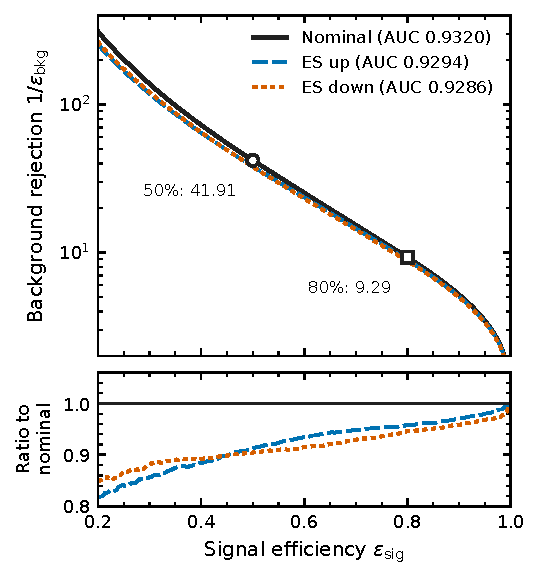
\includegraphics[width=\columnwidth]{figures/figure1_roc.pdf}
  \caption{Receiver-operating-characteristic curve of the frozen tagger on the
    nominal test sample, and on the two cluster energy-scale variations, drawn as
    background rejection $1/\epsilon_{\mathrm{bkg}}$ against signal efficiency
    $\epsilon_{\mathrm{sig}}$ on a logarithmic vertical axis. The horizontal range is
    restricted to $\epsilon_{\mathrm{sig}} > 0.2$, below which the rejection rises
    steeply and carries no information relevant to the working points used here. The
    lower panel gives the ratio of each varied curve to the nominal one on a linear
    axis; on the logarithmic axis above, the three curves are too close to separate by
    eye, and the ratio introduces no quantity that is not already in the upper panel.
    Curves are computed from the frozen prediction files with the unweighted convention
    of Section~\ref{sec:syst}; the areas under the curve quoted in the legend are the
    frozen values, the nominal one as in Table~\ref{tab:nominal-performance} and the
    two varied ones as quoted in Section~\ref{sec:nominal}. Open markers are the two
    working points reported in this paper, labelled with the frozen
    background-rejection values of Table~\ref{tab:nominal-performance} rather than with
    values read off the curve.}
  \label{fig:roc}
\end{figure}

\begin{figure*}[tbp]
  \centering
  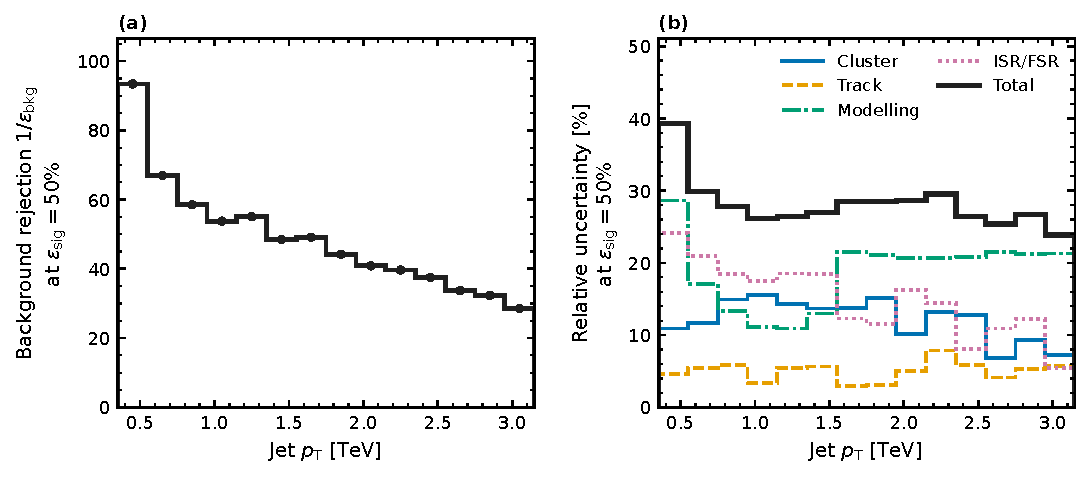
\includegraphics[width=\textwidth]{figures/figure2_performance_systematics.pdf}
  \caption{Tagger performance and its systematic uncertainty as a function of jet
    $\pt$, at $50\%$ signal efficiency throughout, in the fourteen physical
    $200$~GeV bins spanning $350$--$3150$~GeV. \textbf{(a)} Nominal background
    rejection $1/\epsilon_{\mathrm{bkg}}$; markers are bin centres.
    \textbf{(b)} Relative uncertainty on background rejection by category: cluster
    (energy scale envelope combined in quadrature with energy and position
    resolution), track (efficiency and fake-rate envelopes combined in quadrature with
    track bias), modelling (signal and background parton shower and hadronisation), and
    ISR/FSR (the four shower-weight scale envelopes); Total is their quadrature sum.
    The error bars in (a) and the shaded bands in (b) are $\pm1$ standard deviation
    of 100 Poisson bootstrap replicas, drawn around the frozen measured values
    (Section~\ref{sec:precision}); their bin-by-bin values are given in
    Supplementary Table~S8. The step in the modelling curve between the $1.35$--$1.55$~TeV and
    $1.55$--$1.75$~TeV bins is the official extrapolation convention described in
    Section~\ref{sec:syst}: signal modelling is measured only below $1.5$~TeV and is
    held at its maximum measured value from $1.55$~TeV upwards. Bin-by-bin values for
    every component are given in Supplementary Tables~S2 and~S3.}
  \label{fig:perf}
\end{figure*}

\subsection{Systematic uncertainties}
\label{sec:systresults}

Table~\ref{tab:inclusive-systematics-wp50} gives the inclusive breakdown at $50\%$
signal efficiency and Fig.~\ref{fig:perf}(b) its $\pt$ dependence. The total relative
uncertainty on background rejection is $25.83\%$.

Generator modelling dominates at $20.01\%$, and within it the signal generator
comparison (\texttt{ttbar\_herwig} against \texttt{ttbar\_pythia}) contributes
$18.59\%$ against $7.40\%$ for the two background comparisons combined. The ISR/FSR
scale variations follow at $12.04\%$, almost entirely from the signal
final-state-radiation envelope ($11.34\%$); the three remaining scale envelopes ---
signal ISR $0.19\%$, background ISR $1.87\%$ and background FSR $3.60\%$ --- combine to
$4.06\%$ in quadrature, which is not negligible beside the detector terms even though
it is small beside the signal FSR envelope. Detector effects are smaller:
$10.07\%$ for the calorimeter cluster category, of which the energy-scale envelope
alone is $9.58\%$, and $4.51\%$ for tracking, split between the fake-rate
($3.78\%$) and efficiency ($2.47\%$) envelopes with a negligible $0.16\%$ from track
bias.

The $\pt$ dependence in Fig.~\ref{fig:perf}(b) is not flat. The total is largest in the
lowest bin ($39.3\%$), falls to about $26\%$ between $0.95$ and $1.55$~TeV, and rises
again above $1.55$~TeV as the extrapolated signal-modelling term takes over. The
cluster and track curves fluctuate bin to bin at the few-percent level.

The bootstrap of Section~\ref{sec:precision} separates that structure from sample
statistics. In each bin the statistical standard deviation of the total is $1.3$ to
$2.6$ percentage points (Supplementary Table~S8). A $\chi^2$ comparison of each binned
detector curve with a $\pt$-independent constant, treating the fourteen bins as
independent and the bootstrap standard deviations as Gaussian, gives
$\chi^2 = 55.7$ for 13 degrees of freedom for the energy-scale envelope and $45.7$ for
the cluster category, so their $\pt$ dependence is genuine. For the track category it
gives $\chi^2 = 5.4$, and for \texttt{cer}, \texttt{cpos} and track bias $15.9$, $3.4$
and $4.7$: the bin-to-bin fluctuation of these curves is compatible with statistics
alone, and in eight of the fourteen bins the \texttt{cpos} and the track-bias values are
each smaller than their own statistical standard deviation. The values of $\chi^2$ for
these small components are lower than 13 degrees of freedom would make likely, which
is itself a sign that taking the modulus compresses their bin-to-bin scatter; for them
the test is qualitative. Because every component is a
modulus, noise also biases it upward: the replica mean of the binned total lies $0.8$ to
$1.6$ percentage points above the measured value.

Inclusively, the statistical precision is sufficient for nearly every component
(Table~\ref{tab:inclusive-systematics-wp50}). The energy-scale envelope is
$9.58 \pm 0.33\%$, signal modelling $18.59 \pm 0.50\%$, signal FSR
$11.34 \pm 0.64\%$ and the total $25.83 \pm 0.58\%$, and every entry of the table except
two lies at least five standard deviations from zero. Of the two background
modelling comparisons that the table combines, the parton-shower one is
$1.29 \pm 0.40\%$. The exceptions are \texttt{cpos}, at
$1.13 \pm 0.33\%$, and track bias, at $0.16 \pm 0.32\%$ with a replica mean of
$0.45\%$; track bias is consistent with zero and does not meet the documentation's
requirement that the statistical uncertainty be smaller than the difference it
measures~\cite{ATLASGitLab}.

The dependence on the training seed is of the same order as the statistical precision
of the total and smaller than it for the nominal performance. Over six seeds the total
is $26.32 \pm 0.47\%$, ranging from $25.83\%$ to $27.01\%$, and the modelling term
$20.65 \pm 0.43\%$; the frozen seed gives the lowest total and the lowest modelling term of the six,
about one standard deviation below the six-seed means. The two effects
are not independent, since a refitted model places a different set of jets near the
working-point threshold, and we do not combine them. Together they indicate that the
frozen total is determined to about $0.6$ percentage points statistically and a further
$0.5$ from the choice of seed, and none of the conclusions drawn from the budget depends
on either. The per-seed values are listed in Supplementary Table~S9.

% Generated by tables/make_extension_tables.py. The first three columns are
% the frozen layout table verbatim; the last two columns are new.
% Requires \usepackage{booktabs}.
\begin{table*}[tbp]
\centering
\caption{Inclusive relative systematic uncertainties at 50\% signal efficiency. Envelopes are taken before quadrature combination. ``Frozen'' is the frozen result. ``Stat.\ s.d.'' is the standard deviation of the same quantity over 100 Poisson bootstrap replicas in which exactly paired calorimeter jets share their nominal partner's weight. ``Six seeds'' is the mean and standard deviation over six training seeds of the frozen configuration on the same training jets; seed 42 reproduces the frozen column exactly (Section~\ref{sec:precision}).}
\label{tab:inclusive-systematics-wp50}
\begin{tabular}{llrrr}
\toprule
Category & Component & Frozen [\%] & Stat.\ s.d.\ [\%] & Six seeds [\%] \\
\midrule
Cluster & Cluster energy scale & 9.58 & 0.33 & $9.45 \pm 0.11$ \\
Cluster & CER & 2.89 & 0.36 & $2.89 \pm 0.10$ \\
Cluster & CPOS & 1.13 & 0.33 & $0.80 \pm 0.19$ \\
Cluster & Cluster total & 10.07 & 0.43 & $9.91 \pm 0.11$ \\
Track & Track efficiency & 2.47 & 0.45 & $2.26 \pm 0.15$ \\
Track & Fake rate & 3.78 & 0.45 & $3.69 \pm 0.10$ \\
Track & Bias & 0.16 & 0.32 & $0.11 \pm 0.08$ \\
Track & Track total & 4.51 & 0.55 & $4.33 \pm 0.12$ \\
Modelling & Signal modelling & 18.59 & 0.50 & $19.15 \pm 0.43$ \\
Modelling & Background modelling & 7.40 & 0.37 & $7.72 \pm 0.29$ \\
Modelling & Modelling total & 20.01 & 0.49 & $20.65 \pm 0.43$ \\
ISR/FSR & Signal ISR & 0.19 & 0.03 & $0.20 \pm 0.01$ \\
ISR/FSR & Signal FSR & 11.34 & 0.64 & $11.43 \pm 0.33$ \\
ISR/FSR & Background ISR & 1.87 & 0.25 & $1.90 \pm 0.10$ \\
ISR/FSR & Background FSR & 3.60 & 0.51 & $3.85 \pm 0.28$ \\
ISR/FSR & ISR/FSR total & 12.04 & 0.65 & $12.22 \pm 0.37$ \\
Total & Total uncertainty & 25.83 & 0.58 & $26.32 \pm 0.47$ \\
\bottomrule
\end{tabular}
\end{table*}


\subsection{Paired SHAP-Delta}
\label{sec:shapresults}

Fig.~\ref{fig:shap} and Table~\ref{tab:shap-delta-100k} give the paired attribution
result on $100{,}000$ matched pairs per systematic, for the four calorimeter-cluster
variations of Table~\ref{tab:pairing}.

The per-jet attribution drift is concentrated. For the two energy-scale variations the
largest mean $|\Delta\mathrm{SHAP}|$ falls on ECF$_3$ ($0.127$ for \texttt{esup},
$0.132$ for \texttt{esdown}, in margin units), more than twice the next-largest entry,
followed by ECF$_1$, $L_2$, thrust major and $\tau_4^{\mathrm{WTA}}$. \texttt{cer} is
led by ECF$_3$ at about half that size ($0.062$), with $\tau_4^{\mathrm{WTA}}$ close
behind. \texttt{cpos} differs in both size and shape: its largest drift is an order of
magnitude smaller ($\tau_4^{\mathrm{WTA}}$, $0.013$) and the energy correlators no
longer lead. That the two variations which change constituent energies move ECF$_3$ and ECF$_1$
most, while the variation that changes constituent positions does not, is
what one expects from what each variation does to the inputs, and
Section~\ref{sec:degreeresults} measures that input response directly.

Global feature-importance orderings are highly stable under all four variations, and
change only minimally. On the $100{,}000$-pair samples the Spearman correlation between
the nominal and varied orderings is at least $0.986$ across all twelve
systematic-by-class combinations, and is exactly $1$ in eight of them; restricted to
the four all-jet orderings the minimum is $0.993$. The two highest-ranked features are
identical in every case. Movement inside the top four is confined to two adjacent swaps
of ranks three and four, both under \texttt{esdown} --- $L_2$ with thrust major for all
jets, and $L_2$ with $\sqrt{d_{23}}$ for background jets --- and the largest rank change
anywhere is two positions. This is the point of separating the two summaries:
attributions move appreciably for individual jets while the average importance ordering
the model relies on barely moves. Per-feature values of both summaries are given in
Supplementary Table~S6, and the score- and rank-level summaries, which are properties of
a systematic and class subset rather than of a feature, in Supplementary Table~S7.

Score drift, in probability space, is small and class-dependent. Under \texttt{esup}
the mean signed score change is $-0.0029$ for signal and $+0.0055$ for background ---
the two classes move towards each other, the direction consistent with the loss of
background rejection under \texttt{esup} ($8.8\%$ inclusively; the two-sided
energy-scale envelope reported in Table~\ref{tab:inclusive-systematics-wp50} is the
larger \texttt{esdown} value, $9.58\%$). Under \texttt{esdown} both classes move
down, signal further ($-0.0113$) than background ($-0.0045$). \texttt{cer} and
\texttt{cpos} produce shifts an order of magnitude smaller.

The nested $25{,}000$ and $50{,}000$ subsets reproduce the $100{,}000$-jet result
closely: Spearman correlations of the per-feature mean $|\Delta\mathrm{SHAP}|$ against
the full sample are $\ge 0.989$ in every case, and the five leading drift features agree
in 23 of 24 comparisons. Because the smaller sets are nested inside the largest, this is
a convergence check on sample size, not an independent replication, and we present it
as such.

\begin{figure*}[tbp]
  \centering
  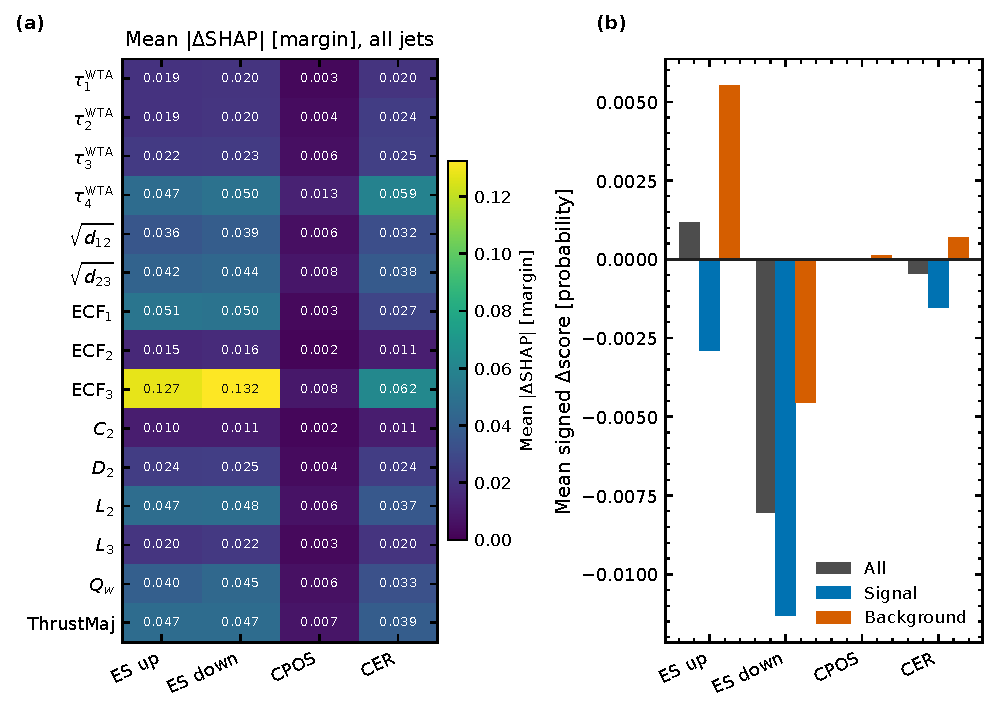
\includegraphics[width=\textwidth]{figures/figure3_shap_delta.pdf}
  \caption{Paired SHAP-Delta for the four calorimeter-cluster variations, on
    $100{,}000$ matched nominal-to-varied jet pairs per systematic. Columns are, in
    order, \texttt{esup} (ES up), \texttt{esdown} (ES down), \texttt{cpos} (cluster
    position resolution) and \texttt{cer} (cluster energy resolution).
    \textbf{(a)} Mean $|\Delta\mathrm{SHAP}|$ per feature over all
    jets, in the additive margin space of the booster; each cell carries its own value
    so that the small entries can be read without the colour scale.
    \textbf{(b)} Mean signed change in classifier score, in probability space, for all
    jets and separately for the signal and background classes. Panel~(b) is a per-jet
    score difference, computed under the same class mask as the corresponding subset,
    and is not derived from panel~(a).}
  \label{fig:shap}
\end{figure*}

% Requires \usepackage{booktabs}.
\begin{table*}[tbp]
\centering
\caption{Final 100k paired SHAP-Delta summary from round 3. Score changes are in probability space; SHAP changes are in XGBoost margin space.}
\label{tab:shap-delta-100k}
\resizebox{\textwidth}{!}{%
\begin{tabular}{lrrrrlr}
\toprule
Systematic & Mean $\Delta$s, all & Mean $\Delta$s, signal & Mean $\Delta$s, background & Mean $|\Delta s|$, all & Leading feature & Leading mean $|\Delta\mathrm{SHAP}|$ \\
\midrule
esup & 0.001164521 & -0.002881727 & 0.00552187 & 0.02799123 & fjet\_ECF3 & 0.1272049 \\
esdown & -0.00805153 & -0.01131766 & -0.004534003 & 0.02917145 & fjet\_ECF3 & 0.1323322 \\
cpos & 3.680653e-05 & -4.375854e-05 & 0.0001235694 & 0.004166955 & fjet\_Tau4\_wta & 0.01281977 \\
cer & -0.0004647173 & -0.001544582 & 0.0006985468 & 0.02119591 & fjet\_ECF3 & 0.06174069 \\
\bottomrule
\end{tabular}%
}
\end{table*}


\subsection{Momentum-scale degree and the scale-free test}
\label{sec:degreeresults}

Table~\ref{tab:feature-response} gives the per-jet response of every input on all
matched pairs, and Supplementary Table~S10 its full distribution. Under \texttt{esup} the summed constituent transverse momentum ECF$_1$
rises by a median $7.41\%$, and the response of every other input is ordered by its degree:
$+4.29\%$ to $+5.48\%$ for the other three quantities with $d=1$, $+12.57\%$ for
ECF$_2$, $+17.63\%$ for ECF$_3$, and between $-1.87\%$ and $+0.28\%$ for the nine
dimensionless ones. \texttt{esdown} mirrors this with opposite sign. The dimensionful
responses are smaller than a uniform rescaling would give ($15.36\%$ for ECF$_2$ and
$23.91\%$ for ECF$_3$), and the dimensionless ones are not exactly zero. Both show that
the variation is not a uniform rescaling of all constituents, which is consistent with
the documentation's description of it as acting on the calorimeter-reconstructed
constituents~\cite{ATLASGitLab}; we have not checked which constituents are left
unscaled. Under \texttt{cer} the median responses vanish but individual
jets move, and ECF$_3$ again has the largest median absolute response of all fifteen
inputs, $4.88\%$, against $3.59\%$ for ECF$_2$ and at most $2.46\%$ for any dimensionless
input. Under \texttt{cpos} no input moves by more than $0.12\%$ in median absolute
value, and ECF$_3$ and $\tau_4^{\mathrm{WTA}}$ respond almost equally ($0.117\%$ and
$0.115\%$).

% Generated by tables/make_extension_tables.py from
% 04_Results/feature_response_round1/feature_response_summary.json.
\begin{table}[tbp]
\centering\footnotesize
\setlength{\tabcolsep}{2.6pt}
\caption{Per-jet response of the fifteen reconstructed inputs to the four exactly paired calorimeter variations, over all matched eligible jet pairs ($4{,}999{,}999$ for \texttt{esup}, \texttt{esdown} and \texttt{cpos}, $4{,}995{,}058$ for \texttt{cer}; the at most 44 pairs per quantity with a non-finite value are left out). $d$ is the degree of each quantity in the constituent four-momenta. The response of a jet is $r = X^{s}/X^{\mathrm{nom}}-1$ for the same physical jet. ``Uniform'' is the response a degree-$d$ quantity would have if every constituent $\pt$ were scaled by the median ECF$_1$ response, $(1.0741)^{d}-1$. For \texttt{cer} and \texttt{cpos}, whose median responses are close to zero, the median absolute response is given instead. All entries are in percent; the full distributions are in Supplementary Table~S10.}
\label{tab:feature-response}
\begin{tabular}{lcrrrrr}
\toprule
 & & \multicolumn{3}{c}{Median $r$ [\%]} & \multicolumn{2}{c}{Median $|r|$ [\%]} \\
\cmidrule(lr){3-5}\cmidrule(lr){6-7}
 & $d$ & \texttt{esup} & Uniform & \texttt{esdown} & \texttt{cer} & \texttt{cpos} \\
\midrule
$\tau_1^{\mathrm{WTA}}$ & 0 & $-0.94$ & $0$ & $+1.08$ & 2.13 & 0.023 \\
$\tau_2^{\mathrm{WTA}}$ & 0 & $-1.45$ & $0$ & $+1.65$ & 2.36 & 0.055 \\
$\tau_3^{\mathrm{WTA}}$ & 0 & $-1.73$ & $0$ & $+1.98$ & 2.41 & 0.090 \\
$\tau_4^{\mathrm{WTA}}$ & 0 & $-1.87$ & $0$ & $+2.14$ & 2.46 & 0.115 \\
$\sqrt{d_{12}}$ & 1 & $+5.42$ & $+7.41$ & $-5.41$ & 2.67 & 0.023 \\
$\sqrt{d_{23}}$ & 1 & $+4.29$ & $+7.41$ & $-4.30$ & 3.20 & 0.035 \\
ECF$_1$ & 1 & $+7.41$ & $+7.41$ & $-7.41$ & 2.14 & 0.001 \\
ECF$_2$ & 2 & $+12.57$ & $+15.36$ & $-11.92$ & 3.59 & 0.027 \\
ECF$_3$ & 3 & $+17.63$ & $+23.91$ & $-15.94$ & 4.88 & 0.117 \\
$C_2$ & 0 & $-0.32$ & $0$ & $+0.37$ & 0.72 & 0.064 \\
$D_2$ & 0 & $+0.28$ & $0$ & $-0.32$ & 1.38 & 0.049 \\
$L_2$ & 0 & $-0.42$ & $0$ & $+0.47$ & 0.94 & 0.042 \\
$L_3$ & 0 & $-1.00$ & $0$ & $+1.13$ & 1.40 & 0.035 \\
$Q_w$ & 1 & $+5.48$ & $+7.41$ & $-5.56$ & 2.27 & 0.041 \\
Thrust major & 0 & $+0.08$ & $0$ & $-0.09$ & 0.33 & 0.013 \\
\bottomrule
\end{tabular}
\end{table}


This accounts for the leading entry of the attribution pattern of
Section~\ref{sec:shapresults}. ECF$_3$, the input of highest degree, is the input whose
value moves most for the same physical jet under the two energy-scale variations and
under \texttt{cer}, and it is the input whose attribution moves most under all three.
It does not account for the rest of the ordering. Under \texttt{esup}, ECF$_2$ has the
second-largest response but almost the smallest attribution drift, while $L_2$ and
thrust major, which move by less than $1\%$, rank third and fourth; under
\texttt{cpos}, where ECF$_3$ and $\tau_4^{\mathrm{WTA}}$ respond almost equally, the
drift is led by $\tau_4^{\mathrm{WTA}}$. The attribution of an input depends on how
much the model relies on it and, through interactions in the trees, on the inputs that
do move, so the per-jet response explains which input leads but not the full
ordering.

The scale-free test asks the same question of the uncertainty budget
(Table~\ref{tab:scale-free}). Restricted to the nine dimensionless inputs, the same
configuration has an energy-scale uncertainty of $2.03 \pm 0.14\%$, against
$9.45 \pm 0.11\%$ with all fifteen inputs, a cluster total of $2.75\%$ against
$9.91\%$, and a modelling term of $6.60\%$ against $20.65\%$, so that the total falls
from $26.32\%$ to $15.80\%$ (six-seed means and standard deviations). The price is
discrimination: the AUC falls from $0.9320$ to $0.8761$ and the background rejection at
$50\%$ signal efficiency from $41.82$ to $18.88$. Of the four categories only ISR/FSR
rises, from $12.22\%$ to $13.81\%$, almost entirely through the signal final-state
radiation envelope, which goes from $11.43\%$ to $13.48\%$. Adding back the five
dimensionful quantities as ratios $X/\mathrm{ECF}_1^{\,d}$, which restores their shape
but not their scale, recovers little: background rejection $19.48$ and total
uncertainty $16.13\%$.

% Generated by tables/make_extension_tables.py from
% 04_Results/tagger_variants_round1/tagger_variants_summary.json.
\begin{table*}[tbp]
\centering
\caption{The same tagger configuration trained on three input sets, each with six training seeds on the same training jets; entries are the mean and standard deviation over the six seeds, evaluated with the frozen uncertainty procedure on the same test and systematic samples. The nine dimensionless inputs are the $d=0$ quantities of Table~\ref{tab:feature-response}. The third set adds the five dimensionful quantities divided by ECF$_1^{\,d}$, which removes their momentum scale but keeps their shape. AUC seed standard deviations are below $5\times10^{-5}$ and are not shown. BR is background rejection at $50\%$ signal efficiency, and every uncertainty is the inclusive relative uncertainty on it, in percent. Per-seed values are in Supplementary Table~S9.}
\label{tab:scale-free}
\resizebox{\textwidth}{!}{%
\begin{tabular}{lrrrrrrrrr}
\toprule
Inputs & $n$ & AUC & BR@50\% & Energy scale & Cluster & Track & Modelling & ISR/FSR & Total \\
\midrule
All fifteen (frozen inputs) & 15 & $0.9320$ & $41.82 \pm 0.07$ & $9.45 \pm 0.11$ & $9.91 \pm 0.11$ & $4.33 \pm 0.12$ & $20.65 \pm 0.43$ & $12.22 \pm 0.37$ & $26.32 \pm 0.47$ \\
Nine dimensionless ($d=0$) & 9 & $0.8761$ & $18.88 \pm 0.02$ & $2.03 \pm 0.14$ & $2.75 \pm 0.18$ & $2.79 \pm 0.13$ & $6.60 \pm 0.22$ & $13.81 \pm 0.16$ & $15.80 \pm 0.19$ \\
Nine $+$ five $X/\mathrm{ECF}_1^{\,d}$ & 14 & $0.8779$ & $19.48 \pm 0.03$ & $2.16 \pm 0.08$ & $2.90 \pm 0.09$ & $2.49 \pm 0.12$ & $6.45 \pm 0.14$ & $14.28 \pm 0.14$ & $16.13 \pm 0.15$ \\
\bottomrule
\end{tabular}%
}
\end{table*}


Within this feature space, then, the discriminating power and the two largest detector
and modelling sensitivities have a common origin: the absolute momentum scale carried by
the six dimensionful inputs. With no explicit jet $\pt$ or mass among the inputs, these
are the only quantities that carry it. They are what the energy-scale variation shifts,
and removing them also reduces the generator-modelling term by a factor of three; we
have not tested why the generator comparison depends on them. We have not separated
how much of that information is jet mass and how much jet $\pt$. The pattern is the
trade-off between accuracy and precision that Ref.~\cite{ATLAS2024} reports between
architectures, seen here inside a single feature space and attributed to specific inputs.

\subsection{Conformal coverage}
\label{sec:conformalresults}

Fig.~\ref{fig:conformal} shows empirical coverage of the class-conditional prediction
sets on the nominal test sample and on all nine detector-systematic samples, using the
thresholds calibrated once on nominal validation data. Unlike the paired analysis of
Section~\ref{sec:shapresults}, this is a dataset-level comparison and needs no pairing,
which is why it covers all nine samples. Full numbers are in Supplementary Table~S4,
and the structure of the prediction sets in Supplementary Table~S5.

The class-conditional coverages are the primary result, and they stay close to target
everywhere: signal coverage ranges from $89.04\%$ (\texttt{esdown}) to $90.12\%$
(\texttt{esup}), and background coverage from $89.61\%$ (\texttt{esup}) to $90.21\%$
(\texttt{esdown}), against the $90\%$ target and against $90.04\%$ and $90.00\%$ on the
nominal test sample. Every deviation from target is within one percentage point. The
largest single deviation is signal coverage under \texttt{esdown}, at $89.04\%$,
followed by signal coverage under \texttt{tfj} at $89.58\%$.

The two energy-scale directions displace the classes in opposite senses, as expected of
a two-sided variation: under \texttt{esup} signal coverage rises to $90.12\%$ while
background coverage falls to $89.61\%$; under \texttt{esdown} signal falls to $89.04\%$
and background rises to $90.21\%$. \texttt{cpos} moves both classes by less than
$0.06$ percentage points, \texttt{bias} by less than $0.03$ and \texttt{tej} by less
than $0.01$ --- consistent with these being the mildest variations in the
background-rejection budget as well.

Overall coverage is reported as a secondary, descriptive number, because it is a
mixture of the two class-conditional values weighted by each sample's class
composition. On the nominal test sample it is $90.021\%$ against the $90\%$ target,
which confirms that the calibration transfers correctly from the validation split to an
independent nominal sample. On the varied samples it ranges from $89.60\%$
(\texttt{esdown}) to $90.02\%$ (\texttt{bias}). For the four track samples the
comparison to the nominal overall value is particularly weak: \texttt{tfl}, for
instance, is $18.5\%$ signal against the nominal $50.5\%$, so its overall coverage of
$89.96\%$ sits much closer to its background-class value than the nominal number does,
and the difference between the two overall figures is mostly a statement about class
mixture rather than about the tracking variation. No sample produces an empty
prediction set, which follows from the overlap of the two acceptance regions noted in
Section~\ref{sec:conformalmethod}, and mean set sizes range from $1.097$ to $1.107$.

One relation we specifically do not assert is a functional link between the mean score
drift of Section~\ref{sec:shapresults} and the coverage change. Coverage depends on the
probability mass near a fixed calibrated threshold, not on the mean of the score
distribution, and the two do not track each other here: \texttt{esup} shifts the mean
signal score down while raising signal coverage. The two diagnostics are reported side
by side because they answer different questions, and they are not even defined over the
same set of samples.

\begin{figure*}[tbp]
  \centering
  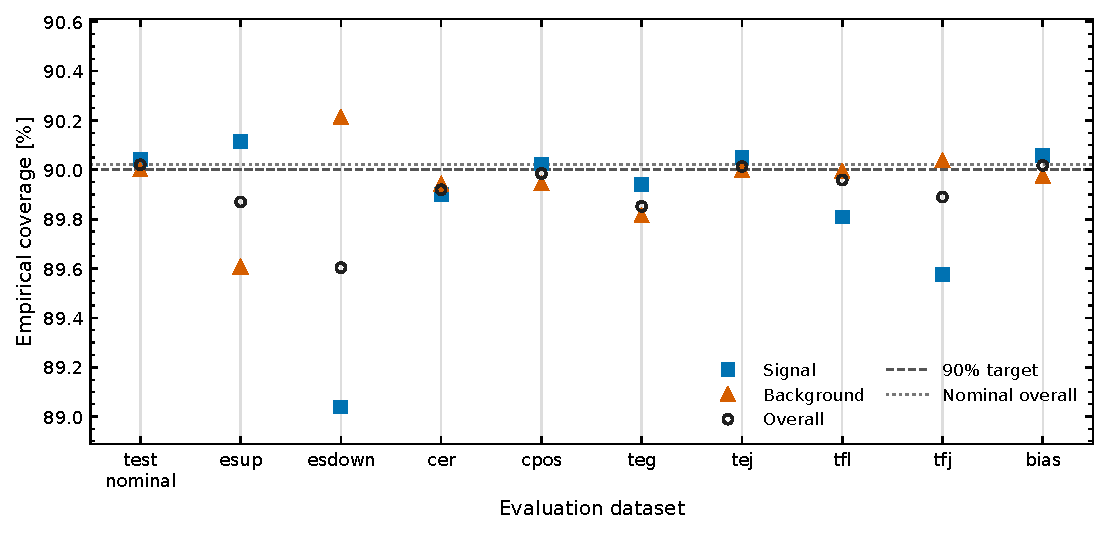
\includegraphics[width=0.86\textwidth]{figures/figure4_conformal_coverage.pdf}
  \caption{Empirical coverage of class-conditional split-conformal prediction sets on
    the nominal test sample and the nine detector-systematic samples. Thresholds were
    calibrated once on the frozen nominal validation split at a $90\%$ target
    (dashed line) and applied unchanged everywhere; the dotted line marks the overall
    coverage measured on the nominal test sample. The horizontal axis is categorical
    and carries no ordering, so the markers are drawn unconnected against light
    vertical guides. The two class-conditional coverages are the primary quantities;
    the overall value is a mixture of them weighted by each sample's class composition,
    which differs strongly between the calorimeter and the track samples. Full values
    are given in Supplementary Table~S4.}
  \label{fig:conformal}
\end{figure*}

% =====================================================================
\section{Discussion}
\label{sec:discussion}

\subsection{What the results support}
\label{sec:support}

Four statements are supported by the frozen artifacts and the extension studies.

The first is about the dataset rather than about any tagger. A robustness study on this
release cannot rely on stored high-level branches for the four validated pairable
detector variations, or read per-event weights as detector systematics. It has to
rebuild the feature space from constituents. We have shown that this can be done
to a median relative accuracy of
better than $5\times10^{-7}$ per quantity, with 43 of the 44 jets carrying a residual
above a $10^{-3}$ relative tolerance traced to information missing from the released
constituents and the remaining one to a reproducible floating-point degeneracy, and we
have applied the frozen reconstruction uniformly to 80.5 million jet entries.

The second is that, for this tagger and this feature space, generator modelling
dominates the systematic budget. At $50\%$ signal efficiency the modelling term is
$20.0\%$ against $10.1\%$ for the calorimeter cluster category and $4.5\%$ for
tracking. Removing the two detector categories entirely would take the total from $25.8\%$ to
$23.4\%$, so on this tagger the leverage sits in the generator comparison rather than in
the detector terms. This ordering is not a statistical accident: the statistical
uncertainty of the modelling term is $0.49\%$ and its spread over training seeds
$0.43\%$.

The third concerns what SHAP and conformal diagnostics add beyond a performance number.
They are sensitive to different things. Attribution drift under the energy-scale
variations is large per jet, concentrated on the energy correlators, and yet barely
moves the importance ordering; conformal coverage under the same variations moves by
less than a percentage point but does so in opposite directions for the two classes.
Neither of these is visible in AUC, which changes by $0.003$ between nominal and
\texttt{esup}. We regard both as diagnostics that describe how a classifier's behaviour
shifts, not as significance tests.

The fourth concerns where this tagger's sensitivity comes from. The inputs that respond
most to the calorimeter energy scale are those of highest degree in the constituent
momenta, the largest attribution drift falls on the one of highest degree, and removing the absolute momentum scale
from the inputs removes most of the energy-scale and modelling uncertainty together with
more than half of the background rejection. These are measurements on one model class
and one feature space. The degree of each input, however, is a property of its
definition rather than of gradient boosting, so the same input-level reasoning applies
to any tagger built on these quantities, although we have not tested how other
architectures weigh them.

\subsection{Limitations}
\label{sec:limitations}

The training sample is the clearest limitation. The classifier was developed from a
five-million-jet nominal subset taken from the first fifty released
\texttt{train\_nominal} files, of which $4{,}499{,}612$ jets were used for fitting and
$500{,}385$ held out. The released training partition is much larger, and the files were
taken as a contiguous block rather than a random draw across the partition; we did not
demonstrate that this block is representative of the whole, and we did not run a
training-size scan. The size is close to the six million jets of the reference training
script, but the dataset documentation states that state-of-the-art performance requires
the entire partition~\cite{ATLASGitLab}. The gap to the published hlDNN reference in
Table~\ref{tab:nominal-performance} is therefore not attributable to any single cause,
and we do not attempt to decompose it.

The two diagnostics have different scope, and neither should be read as covering the
other's samples. Paired SHAP-Delta covers four of the nine detector systematics, the
calorimeter-cluster variations that pair jet-by-jet; that restriction is forced by the
data, as Section~\ref{sec:shapmethod} and Table~\ref{tab:pairing} document, and it means
the attribution results speak only to those four. Conformal coverage covers all ten
evaluated samples, but it does so at the level of whole datasets rather than matched
jets, so a coverage difference between a varied sample and nominal is a difference
between two populations and not a per-jet effect. Extending the \emph{paired}
diagnostics to the tracking systematics would require a release in which those samples
are re-simulations of the same jets.

The SHAP results are for one model. TreeSHAP is exact for the fitted trees, so there is
no attribution-estimator uncertainty, but the attributions themselves depend on the
training sample, the seed and the hyperparameters, and we quantify only the dependence
on the evaluation sample size; the six-seed study of Section~\ref{sec:precision} covers
performance and uncertainties, not attributions. Carrying the same paired construction to a second
architecture would test how much of the pattern is a property of the feature space
rather than of gradient boosting.

The conformal results are diagnostic, not inferential. Coverage was measured under
distribution shift with thresholds calibrated on nominal data, a setting in which the
conformal guarantee does not formally hold~\cite{Tibshirani2019}. We report empirical
coverage and its deviation; we do not attach a confidence statement to it, and the
deviations we observe are small enough that we would not read a physical claim into
their ordering.

The statistical uncertainties of this paper describe the finite size of the evaluation
samples. The six-seed study varies the training seed but not the training jets, so the
statistical uncertainty of the training sample itself is not covered, and a comparison
across disjoint training blocks remains to be done. Because each uncertainty component
is a modulus, its bootstrap distribution is skewed when the component is small, and the
standard deviations quoted for \texttt{cpos}, track bias and the smaller binned entries
indicate a size rather than a Gaussian error. The input-set variants have only the
six-seed spread and no bootstrap of their own. Their differences from the full tagger
are many times the statistical precision of the frozen result, but the small difference
between the uncertainties of the two reduced input sets should not be interpreted.

Finally, the binned uncertainty of Fig.~\ref{fig:perf}(b) covers $350$--$3150$~GeV, the
range the reference implementation defines. That range holds $8{,}959{,}008$ of the
$10{,}306{,}812$ eligible test jets, or $86.9\%$; the remaining $13.1\%$ enter the
inclusive numbers but no $\pt$ bin, and they are signal-enriched ($61.8\%$ signal,
against $48.8\%$ inside the binning and $50.5\%$ overall), so the binned and inclusive
numbers are not measurements of the same jet population. The $1.35$--$1.55$~TeV
interval carries the official extrapolation convention rather than a measurement of
its own.

% =====================================================================
\section{Conclusion}
\label{sec:conclusion}

We have rebuilt the fifteen-variable high-level feature space of the ATLAS top-tagging
open dataset from the released jet constituents. For the four exactly pairable
calorimeter variations, the stored high-level branches remain nominal despite
constituent changes; the per-event weight array holds theory rather than detector
variations. The
reconstruction closes against the stored nominal branches to a median relative accuracy
between $2.5\times10^{-8}$ and $4.8\times10^{-7}$ per quantity, with $0.072\%$ of
quantity--jet comparisons outside a $10^{-3}$ tolerance. Those residuals fall on 44
jets, of which 43 are information-loss cases and one is a reproducible floating-point
degeneracy; no proven formula or implementation mismatch was found and no jet was left
unresolved. The reconstruction was frozen and applied to 80{,}481{,}421 jet entries
across seventeen samples.

An XGBoost tagger developed from a five-million-jet nominal subset --- $4{,}499{,}612$
jets for fitting, $500{,}385$ held out --- reaches an unweighted AUC of $0.9320$,
accuracy $0.8559$, and background rejection $41.91$ at $50\%$ signal efficiency on
10{,}306{,}812 test jets. Evaluated with the procedure the record prescribes, the total
relative systematic uncertainty on background rejection is $25.8\%$: generator
modelling $20.0\%$, ISR/FSR scales $12.0\%$, calorimeter clusters $10.1\%$, tracking
$4.5\%$. A bootstrap that preserves the jet-by-jet pairing of the calorimeter
variations gives the total a statistical uncertainty of $0.6$ percentage points, and six
training seeds spread it by $0.5$; every inclusive entry of the uncertainty table except \texttt{cpos}
and track bias is at least five statistical standard deviations from zero, and the $\pt$ dependence of
the energy-scale and cluster terms is genuine while that of the track terms is compatible
with statistics. The published ATLAS high-level network is quoted alongside only as an
external reference in the same feature space.

On the four calorimeter-cluster variations that pair jet-by-jet with the nominal sample,
paired TreeSHAP attribution drift concentrates on ECF$_3$ for the energy-scale and
energy-resolution variations, followed by ECF$_1$ and $L_2$ under the energy scale and
by $\tau_4^{\mathrm{WTA}}$ under the energy resolution, and on $\tau_4^{\mathrm{WTA}}$
at an order of magnitude smaller size for the position variation, while global importance rankings change minimally: the Spearman correlation
between nominal and varied orderings is at least $0.993$ for all-jet rankings and at
least $0.986$ across every systematic-by-class combination. Class-conditional conformal
prediction sets calibrated once on nominal validation data and applied unchanged to the
nominal test sample and all nine detector-systematic samples retain class-conditional
coverage within one percentage point of the $90\%$ target throughout, with the two
energy-scale directions displacing the signal and background classes in opposite senses.

The leading attribution drift follows the degree of each input in the constituent
momenta: under \texttt{esup} ECF$_3$, of degree three, moves by a median $17.6\%$ per jet,
against $7.4\%$ for the summed constituent momentum and less than $2\%$ for every
dimensionless input. Retraining on the nine dimensionless inputs lowers the six-seed
mean total uncertainty from $26.3\%$ to $15.8\%$, through the energy-scale and modelling terms, but
lowers background rejection from $41.8$ to $18.9$, so within this feature space the
discrimination and the leading sensitivities share one origin, the absolute momentum
scale of the dimensionful inputs.

The reading we would defend is narrow. A tagger's response to a systematic variation has
structure that a single performance number does not show, and on a public dataset that
structure can be measured jet-by-jet once the feature space is reconstructed correctly.

% =====================================================================
\section*{Statements and declarations}

\subsection*{Data Availability Statement}

This manuscript has associated data in a data repository. [Authors' comment: This study
analyses the ATLAS top tagging open data set with systematic uncertainties, CERN Open Data
Portal Record 80030, \url{https://doi.org/10.7483/OPENDATA.ATLAS.SOAY.LABE}.]

\subsection*{Code Availability Statement}

This manuscript has associated code/software in a data repository. [Authors' comment:
The analysis code, the trained tagger and the frozen results quoted in this paper are
publicly available at
\url{https://github.com/adeelrahmat64-beep/atlas80030-tagger-robustness}. Release
v1.1.0 adds the scripts and outputs of the statistical-precision, training-seed and
input-degree studies (\texttt{uncertainty\_chain.py}, \texttt{stat\_bootstrap.py},
\texttt{tagger\_variants.py} and \texttt{feature\_response.py}) to the first release,
v1.0.0 (\url{https://doi.org/10.5281/zenodo.23083866}). Every release is archived on
Zenodo under the concept DOI \url{https://doi.org/10.5281/zenodo.23083865}, which
always resolves to the latest version.]

\section*{Acknowledgements}

The authors thank the ATLAS Collaboration and the CERN Open Data Portal for making
Record 80030 publicly available.

% =====================================================================
\begin{thebibliography}{99}

\bibitem{Evans2008}
L.~Evans and P.~Bryant,
\emph{LHC machine},
J. Instrum. \textbf{3} (2008) S08001,
\url{https://doi.org/10.1088/1748-0221/3/08/S08001}.

\bibitem{PDG2024}
Particle Data Group (S.~Navas et al.),
\emph{Review of particle physics},
Phys. Rev. D \textbf{110} (2024) 030001,
\url{https://doi.org/10.1103/PhysRevD.110.030001}.

\bibitem{Thaler2011}
J.~Thaler and K.~Van~Tilburg,
\emph{Identifying boosted objects with $N$-subjettiness},
J. High Energy Phys. \textbf{03} (2011) 015,
\url{https://doi.org/10.1007/JHEP03(2011)015},
arXiv:1011.2268.

\bibitem{Thaler2012}
J.~Thaler and K.~Van~Tilburg,
\emph{Maximizing boosted top identification by minimizing $N$-subjettiness},
J. High Energy Phys. \textbf{02} (2012) 093,
\url{https://doi.org/10.1007/JHEP02(2012)093},
arXiv:1108.2701.

\bibitem{Larkoski2013}
A.~J.~Larkoski, G.~P.~Salam, and J.~Thaler,
\emph{Energy correlation functions for jet substructure},
J. High Energy Phys. \textbf{06} (2013) 108,
\url{https://doi.org/10.1007/JHEP06(2013)108},
arXiv:1305.0007.

\bibitem{Kasieczka2019}
G.~Kasieczka et al.,
\emph{The machine learning landscape of top taggers},
SciPost Phys. \textbf{7} (2019) 014,
\url{https://doi.org/10.21468/SciPostPhys.7.1.014},
arXiv:1902.09914.

\bibitem{Qu2020}
H.~Qu and L.~Gouskos,
\emph{ParticleNet: jet tagging via particle clouds},
Phys. Rev. D \textbf{101} (2020) 056019,
\url{https://doi.org/10.1103/PhysRevD.101.056019},
arXiv:1902.08570.

\bibitem{Komiske2019}
P.~T.~Komiske, E.~M.~Metodiev, and J.~Thaler,
\emph{Energy flow networks: deep sets for particle jets},
J. High Energy Phys. \textbf{01} (2019) 121,
\url{https://doi.org/10.1007/JHEP01(2019)121},
arXiv:1810.05165.

\bibitem{Larkoski2020}
A.~J.~Larkoski, I.~Moult, and B.~Nachman,
\emph{Jet substructure at the Large Hadron Collider: a review of recent advances in
theory and machine learning},
Phys. Rep. \textbf{841} (2020) 1--63,
\url{https://doi.org/10.1016/j.physrep.2019.11.001},
arXiv:1709.04464.

\bibitem{Guest2018}
D.~Guest, K.~Cranmer, and D.~Whiteson,
\emph{Deep learning and its application to LHC physics},
Annu. Rev. Nucl. Part. Sci. \textbf{68} (2018) 161--181,
\url{https://doi.org/10.1146/annurev-nucl-101917-021019},
arXiv:1806.11484.

\bibitem{ATLAS2024}
ATLAS Collaboration,
\emph{Accuracy versus precision in boosted top tagging with the ATLAS detector},
J. Instrum. \textbf{19} (2024) P08018,
\url{https://doi.org/10.1088/1748-0221/19/08/P08018},
arXiv:2407.20127.

\bibitem{CMS2020}
CMS Collaboration,
\emph{Identification of heavy, energetic, hadronically decaying particles using
machine-learning techniques},
J. Instrum. \textbf{15} (2020) P06005,
\url{https://doi.org/10.1088/1748-0221/15/06/P06005},
arXiv:2004.08262.

\bibitem{ATLASOpenData2024}
ATLAS Collaboration,
\emph{ATLAS top tagging open data set with systematic uncertainties},
CERN Open Data Portal, Record 80030 (2024),
\url{https://doi.org/10.7483/OPENDATA.ATLAS.SOAY.LABE}.

\bibitem{Chen2016}
T.~Chen and C.~Guestrin,
\emph{XGBoost: a scalable tree boosting system},
in: Proceedings of the 22nd ACM SIGKDD International Conference on Knowledge Discovery
and Data Mining (2016) 785--794,
\url{https://doi.org/10.1145/2939672.2939785}.

\bibitem{Friedman2001}
J.~H.~Friedman,
\emph{Greedy function approximation: a gradient boosting machine},
Ann. Stat. \textbf{29} (2001) 1189--1232,
\url{https://doi.org/10.1214/aos/1013203451}.

\bibitem{Lundberg2017}
S.~M.~Lundberg and S.-I.~Lee,
\emph{A unified approach to interpreting model predictions},
Adv. Neural Inf. Process. Syst. \textbf{30} (2017) 4765--4774,
arXiv:1705.07874.

\bibitem{Lundberg2020trees}
S.~M.~Lundberg et al.,
\emph{From local explanations to global understanding with explainable AI for trees},
Nat. Mach. Intell. \textbf{2} (2020) 56--67,
\url{https://doi.org/10.1038/s42256-019-0138-9}.

\bibitem{Vovk2005}
V.~Vovk, A.~Gammerman, and G.~Shafer,
\emph{Algorithmic Learning in a Random World},
Springer, New York (2005),
\url{https://doi.org/10.1007/b106715}.

\bibitem{Angelopoulos2023}
A.~N.~Angelopoulos and S.~Bates,
\emph{Conformal prediction: a gentle introduction},
Found. Trends Mach. Learn. \textbf{16} (2023) 494--591,
\url{https://doi.org/10.1561/2200000101},
arXiv:2107.07511.

\bibitem{Sahu2024}
R.~Sahu and K.~Ghosh,
\emph{ML-based top taggers: performance, uncertainty and impact of tower and tracker
data integration},
SciPost Phys. \textbf{17} (2024) 166,
\url{https://doi.org/10.21468/SciPostPhys.17.6.166},
arXiv:2309.01568.

\bibitem{Bhattacherjee2024}
B.~Bhattacherjee, C.~Bose, A.~Chakraborty, and R.~Sengupta,
\emph{Boosted top tagging and its interpretation using Shapley values},
Eur. Phys. J. Plus \textbf{139} (2024) 1131,
\url{https://doi.org/10.1140/epjp/s13360-024-05910-9},
arXiv:2212.11606.

\bibitem{Araz2025}
J.~Y.~Araz and M.~Spannowsky,
\emph{Another fit bites the dust: conformal prediction as a calibration standard for
machine learning in high-energy physics},
arXiv:2512.17048 (2025),
\url{https://doi.org/10.48550/arXiv.2512.17048}.

\bibitem{ATLASDetector2008}
ATLAS Collaboration,
\emph{The ATLAS experiment at the CERN Large Hadron Collider},
J. Instrum. \textbf{3} (2008) S08003,
\url{https://doi.org/10.1088/1748-0221/3/08/S08003}.

\bibitem{Agostinelli2003}
S.~Agostinelli et al.,
\emph{GEANT4 -- a simulation toolkit},
Nucl. Instrum. Methods Phys. Res. A \textbf{506} (2003) 250--303,
\url{https://doi.org/10.1016/S0168-9002(03)01368-8}.

\bibitem{Sjostrand2015}
T.~Sj\"{o}strand et al.,
\emph{An introduction to PYTHIA 8.2},
Comput. Phys. Commun. \textbf{191} (2015) 159--177,
\url{https://doi.org/10.1016/j.cpc.2015.01.024},
arXiv:1410.3012.

\bibitem{Cacciari2008anti}
M.~Cacciari, G.~P.~Salam, and G.~Soyez,
\emph{The anti-$k_\mathrm{T}$ jet clustering algorithm},
J. High Energy Phys. \textbf{04} (2008) 063,
\url{https://doi.org/10.1088/1126-6708/2008/04/063},
arXiv:0802.1189.

\bibitem{Cacciari2012fastjet}
M.~Cacciari, G.~P.~Salam, and G.~Soyez,
\emph{FastJet user manual},
Eur. Phys. J. C \textbf{72} (2012) 1896,
\url{https://doi.org/10.1140/epjc/s10052-012-1896-2},
arXiv:1111.6097.

\bibitem{Bellm2016}
J.~Bellm et al.,
\emph{Herwig 7.0/Herwig++ 3.0 release note},
Eur. Phys. J. C \textbf{76} (2016) 196,
\url{https://doi.org/10.1140/epjc/s10052-016-4018-8},
arXiv:1512.01178.

\bibitem{Bothmann2019}
E.~Bothmann et al. (Sherpa Collaboration),
\emph{Event generation with Sherpa 2.2},
SciPost Phys. \textbf{7} (2019) 034,
\url{https://doi.org/10.21468/SciPostPhys.7.3.034},
arXiv:1905.09127.

\bibitem{ATLASGitLab}
ATLAS Collaboration,
\emph{ATLAS top tagging open data: reference analysis software and documentation (README.md)},
commit \texttt{5bc3c8d70cf8736d24b\linebreak[0]969972a3dd365017a9e24},
\url{https://gitlab.cern.ch/atlas/ATLAS-top-tagging-open-data/-/tree/%
5bc3c8d70cf8736d24b969972a3dd365017a9e24}
[accessed September and October 2026].

\bibitem{Larkoski2014WTA}
A.~J.~Larkoski, D.~Neill, and J.~Thaler,
\emph{Jet shapes with the broadening axis},
J. High Energy Phys. \textbf{04} (2014) 017,
\url{https://doi.org/10.1007/JHEP04(2014)017},
arXiv:1401.2158.

\bibitem{Thaler2008}
J.~Thaler and L.-T.~Wang,
\emph{Strategies to identify boosted tops},
J. High Energy Phys. \textbf{07} (2008) 092,
\url{https://doi.org/10.1088/1126-6708/2008/07/092},
arXiv:0806.0023.

\bibitem{Larkoski2014PC}
A.~J.~Larkoski, I.~Moult, and D.~Neill,
\emph{Power counting to better jet observables},
J. High Energy Phys. \textbf{12} (2014) 009,
\url{https://doi.org/10.1007/JHEP12(2014)009},
arXiv:1409.6298.

\bibitem{Larkoski2016D2}
A.~J.~Larkoski, I.~Moult, and D.~Neill,
\emph{Analytic boosted boson discrimination},
J. High Energy Phys. \textbf{05} (2016) 117,
\url{https://doi.org/10.1007/JHEP05(2016)117},
arXiv:1507.03018.

\bibitem{Moult2016}
I.~Moult, L.~Necib, and J.~Thaler,
\emph{New angles on energy correlation functions},
J. High Energy Phys. \textbf{12} (2016) 153,
\url{https://doi.org/10.1007/JHEP12(2016)153},
arXiv:1609.07483.

\bibitem{ATLASPub2021}
ATLAS Collaboration,
\emph{Identification of hadronically-decaying top quarks using UFO jets with ATLAS in
Run 2},
ATL-PHYS-PUB-2021-028, CERN, Geneva (2021),
\url{https://cds.cern.ch/record/2776782}.

\bibitem{Kaplan2008}
D.~E.~Kaplan, K.~Rehermann, M.~D.~Schwartz, and B.~Tweedie,
\emph{Top tagging: a method for identifying boosted hadronically decaying top quarks},
Phys. Rev. Lett. \textbf{101} (2008) 142001,
\url{https://doi.org/10.1103/PhysRevLett.101.142001},
arXiv:0806.0848.

\bibitem{Chen2012}
C.~Chen,
\emph{New approach to identifying boosted hadronically-decaying particle using jet
substructure in its center-of-mass frame},
Phys. Rev. D \textbf{85} (2012) 034007,
\url{https://doi.org/10.1103/PhysRevD.85.034007},
arXiv:1112.2567.

\bibitem{Harris2020}
C.~R.~Harris et al.,
\emph{Array programming with NumPy},
Nature \textbf{585} (2020) 357--362,
\url{https://doi.org/10.1038/s41586-020-2649-2}.

\bibitem{Lam2015}
S.~K.~Lam, A.~Pitrou, and S.~Seibert,
\emph{Numba: a LLVM-based Python JIT compiler},
in: Proceedings of the Second Workshop on the LLVM Compiler Infrastructure in HPC
(2015) 7:1--7:6,
\url{https://doi.org/10.1145/2833157.2833162}.

\bibitem{Virtanen2020}
P.~Virtanen et al.,
\emph{SciPy 1.0: fundamental algorithms for scientific computing in Python},
Nat. Methods \textbf{17} (2020) 261--272,
\url{https://doi.org/10.1038/s41592-019-0686-2}.

\bibitem{Steele2014}
G.~L.~Steele~Jr., D.~Lea, and C.~H.~Flood,
\emph{Fast splittable pseudorandom number generators},
in: Proceedings of the 2014 ACM International Conference on Object Oriented
Programming Systems Languages \& Applications (OOPSLA) (2014) 453--472,
\url{https://doi.org/10.1145/2660193.2660195}.

\bibitem{Pedregosa2011}
F.~Pedregosa et al.,
\emph{Scikit-learn: machine learning in Python},
J. Mach. Learn. Res. \textbf{12} (2011) 2825--2830.

\bibitem{Efron1979}
B.~Efron,
\emph{Bootstrap methods: another look at the jackknife},
Ann. Stat. \textbf{7} (1979) 1--26,
\url{https://doi.org/10.1214/aos/1176344552}.

\bibitem{Hanley2006}
J.~A.~Hanley and B.~MacGibbon,
\emph{Creating non-parametric bootstrap samples using Poisson frequencies},
Comput. Methods Programs Biomed. \textbf{83} (2006) 57--62,
\url{https://doi.org/10.1016/j.cmpb.2006.04.006}.

\bibitem{Tibshirani2019}
R.~J.~Tibshirani, R.~F.~Barber, E.~J.~Cand\`{e}s, and A.~Ramdas,
\emph{Conformal prediction under covariate shift},
Adv. Neural Inf. Process. Syst. \textbf{32} (2019),
arXiv:1904.06019.

\end{thebibliography}

\end{document}
